\documentclass[10pt, aspectratio=169]{beamer}
\usetheme{Madrid}
\usepackage[spanish]{babel}
\usepackage[utf8]{inputenc}
\usepackage{pgfplots}
\pgfplotsset{compat=1.18}

% --- PALETA INSTITUCIONAL UG ---
\definecolor{AzulUG}{HTML}{002855}
\definecolor{DoradoUG}{HTML}{C59B27}

\setbeamercolor{structure}{fg=AzulUG}
\setbeamercolor{palette primary}{bg=AzulUG, fg=white}
\setbeamercolor{palette secondary}{bg=AzulUG!90, fg=white}
\setbeamercolor{palette tertiary}{bg=AzulUG!80, fg=white}
\setbeamercolor{titlelike}{parent=palette primary, fg=white}

% --- DATOS DE LA PRESENTACIÓN ---
\title[El Landscape, el Swampland y las Metaheurísticas]{El Landscape, el Swampland y las Metaheurísticas}
\subtitle{Presentación de Trabajo de Investigación}

\author[B. Marquez-Salazar et al.]{Brandon Marquez-Salazar \and Angel Diaz-Pacheco \and Cesar Damian}
\institute[UG]{
  División de Ingenierías Campus Irapuato-Salamanca\\
  \textbf{Universidad de Guanajuato}\\
  Salamanca, Guanajuato, México
}
\date{}

\begin{document}

\begin{frame}
  \maketitle
\end{frame}

\begin{frame}{1. ¿Qué son el Landscape y el Swampland?}
  \begin{columns}
    \column{0.48\textwidth}
    \begin{block}{Geometría de las Soluciones}
      El \textbf{Landscape} engloba las configuraciones con vacíos estables y físicamente consistentes. 

      Alrededor yace el \textbf{Swampland}: una vasta «bruma» de soluciones que violan principios de gravedad cuántica.
    \end{block}

    \begin{alertblock}{Composición del hiperespacio según las conjeturas del Swampland}
      Preponderancia de estados de energía negativa frente a la escasez de vacíos cosmológicos de Sitter.
    \end{alertblock}

    \column{0.52\textwidth}
    \centering
    \begin{tikzpicture}[scale=0.85]
      \begin{axis}[
        domain=-2.5:2.5,
        domain y=-2.5:2.5,
        view={0}{90}, % Vista superior
        axis lines=none,
        ticks=none,
        % Colormap sesgado: Predominio de Cyan Oscuro con picos de Cyan Claro y destellos de Amarillo
        colormap={custom_swampland}{
          rgb255(0.0cm)=(0, 25, 55);     % Mayoría del espacio: Cyan muy oscuro
          rgb255(1.6cm)=(10, 75, 125);   % Fondo base: Cyan oscuro
          rgb255(2.4cm)=(80, 215, 245);  % Picos aislados: Cyan claro (AdS estable)
          rgb255(2.8cm)=(165, 115, 0);   % Transición rápida: Ámbar (dS inestable)
          rgb255(3.0cm)=(255, 235, 90)   % Puntos mínimos/escasos: Amarillo claro (dS estable)
        }
      ]
        % Superficie aperiódica y caótica (armónicos cruzados no enteros)
        \addplot3[
          surf,
          shader=interp,
          samples=50
        ] {
          sin(deg(2.3*x + 1.7*y + 1.1)) * cos(deg(3.1*x - 1.4*y)) 
          + 0.5 * sin(deg(1.9*x*y + 2.4)) 
          - 0.4 * cos(deg(4.2*x - 0.7*y^2))
        };

        % Anotación discreta en el fondo
        \node[font=\tiny\bfseries, color=white!70] at (axis cs:-1.7,-2.0,0) {SWAMPLAND};
      \end{axis}
    \end{tikzpicture}
  \end{columns}
\end{frame}

\begin{frame}{1. La Función de Potencial Efectivo (\(V_{\text{eff}}\))}
  \begin{block}{Formulación Analítica en Compactaciones (Tipo IIB)}
    El potencial escalar \(V_{\text{eff}}\) en función del axio-dilatón (\(s\)) y el módulo de volumen (\(\tau\)) se expresa como:
    \begin{equation*}
      V_{\text{eff}} = \frac{A_{H_3} s}{\tau^3} + \frac{A_{F_3}}{s \tau^3} + \frac{A_{F_5}}{\tau^4} + \frac{A_3 \mathcal{N}_3}{\tau^3} + \frac{A_{\widehat{D5}}}{s^{1/2} \tau^{5/2}}
    \end{equation*}
  \end{block}

  \begin{columns}
    \column{0.50\textwidth}
    \begin{block}{Estructura del Potencial}
      \begin{itemize}
        \item \textbf{Módulos de compactación:} \(s, \tau > 0\).
        \item \textbf{Coeficientes de flujo:} \(A_{H_3}, A_{F_3}, A_{F_5}, A_3 \mathcal{N}_3, A_{\widehat{D5}}\).
      \end{itemize}
    \end{block}

    \column{0.50\textwidth}
    \begin{alertblock}{Espacio de Búsqueda}
      El problema de optimización se define sobre el vector de parámetros libres:
      \begin{center}
        \(\mathbf{x} = \{A_{H_3}, A_{F_3}, A_{F_5}, A_3 \mathcal{N}_3, A_{\widehat{D5}}\}\)
      \end{center}
    \end{alertblock}
  \end{columns}
\end{frame}

\begin{frame}{1. Potencial Efectivo y Función de Aptitud (\textit{Fitness})}
  \begin{columns}
    \column{0.50\textwidth}
    \begin{block}{Penalizaciones Locales y Físicas}
      \begin{itemize}
        \item \textbf{Extremos de \(V_{\text{eff}}\):} \(\pi_1(x) = |\nabla V_{\text{eff}}(x)|^2\).
        \item \textbf{Penalización AdS:} \(\pi_2(x) = |V_{\text{eff}}(x)| - V_{\text{eff}}(x)\).
        \item \textbf{Mecanismo elevador \(\widehat{D5}\):} \(\pi_5(x) = |A_{\widehat{D5}}| - A_{\widehat{D5}}\).
      \end{itemize}
    \end{block}

    \column{0.50\textwidth}
    \begin{alertblock}{Estabilidad por Matriz Hessiana (\(H\))}
      Para evitar taquiones mediante la matriz de masa \(H\):
      \begin{itemize}
        \item \textbf{Traza de \(H\):} \(\pi_3(x) = |\text{tr}(H)| - \text{tr}(H)\).
        \item \textbf{Discriminante:} \(\pi_4(x) = |\Delta| - \Delta\), con:
        \begin{equation*}
          \Delta = \det(H) - \frac{1}{4}\text{tr}^2(H)
        \end{equation*}
      \end{itemize}
    \end{alertblock}
  \end{columns}
\end{frame}

\begin{frame}{2. Teorema de No Free Lunch (NFLT) y Motivación}
  \begin{block}{Teorema de No Free Lunch (NFLT)}
    Demostrado por Wolpert y Macready, establece que ninguna metaheurística es inherentemente superior al resto.
  \end{block}

  \vspace{0.3cm}

  \begin{block}{Evolución Metodológica}
    En la propuesta inicial donde se definió la función potencial aquí expuesta, se utilizó \textit{Simulated Annealing} (SA).
    Sin embargo, debido a la naturaleza del potencia, se optó por metaheurísticas poblacionales para aprovechar sus capacidades
    de exploración.

    \vspace{0.2cm}

    Con este enfoque, se abordó el primer experimento empleando Algoritmos Genéticos (GA), mientras que para el segundo
    experimento se seleccionaron AIW-PSO e IWO.
  \end{block}
\end{frame}

\begin{frame}{3. Experimento 1: Parámetros Óptimos del GA}
  \begin{columns}
    \column{0.45\textwidth}
    \begin{block}{Metodología y Análisis}
      Evaluación sistemática de la configuración del Algoritmo Genético para maximizar la exploración del espacio de búsqueda.
      
      \vspace{0.2cm}
      
      Se analizaron \textbf{11,979 puntos críticos} identificados, comparando la distribución y estabilidad de las soluciones al
      incluir y omitir el término \(A_{\widehat{D5}}\).
    \end{block}

    \column{0.55\textwidth}
    \begin{figure}
      \centering
      % Reemplaza "ruta/a/tu_grafica_exp1.pdf" por la imagen de tu gráfica
      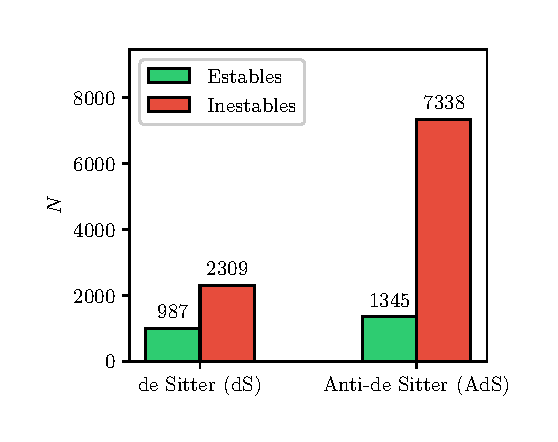
\includegraphics[width=\textwidth, height=0.65\textheight, keepaspectratio]{./Histograma129032026.eps}
      \caption{\small Resultados del GA.}
    \end{figure}
  \end{columns}
\end{frame}

\begin{frame}{4. Experimento 2: Benchmark AIW-PSO frente a IWO}
  \begin{columns}
    \column{0.48\textwidth}
    \begin{block}{Metodología y Evaluación Multicriterio}
      A partir de 88 configuraciones de módulos \((s, \tau)\) fijadas desde un dataset previo, se ejecutaron 100 optimizaciones por configuración. Esto generó 8,800 puntos críticos por cada una de las 32 instancias evaluadas de los optimizadores.

      \vspace{0.2cm}

      El contraste se realizó mediante 7 momentos estadísticos, jerarquizados finalmente a través de un conteo de Borda uniformemente pesado.
    \end{block}

    \column{0.52\textwidth}
    \begin{figure}
      \centering
      % Reemplaza con la ruta de tu gráfica para el Exp 2
      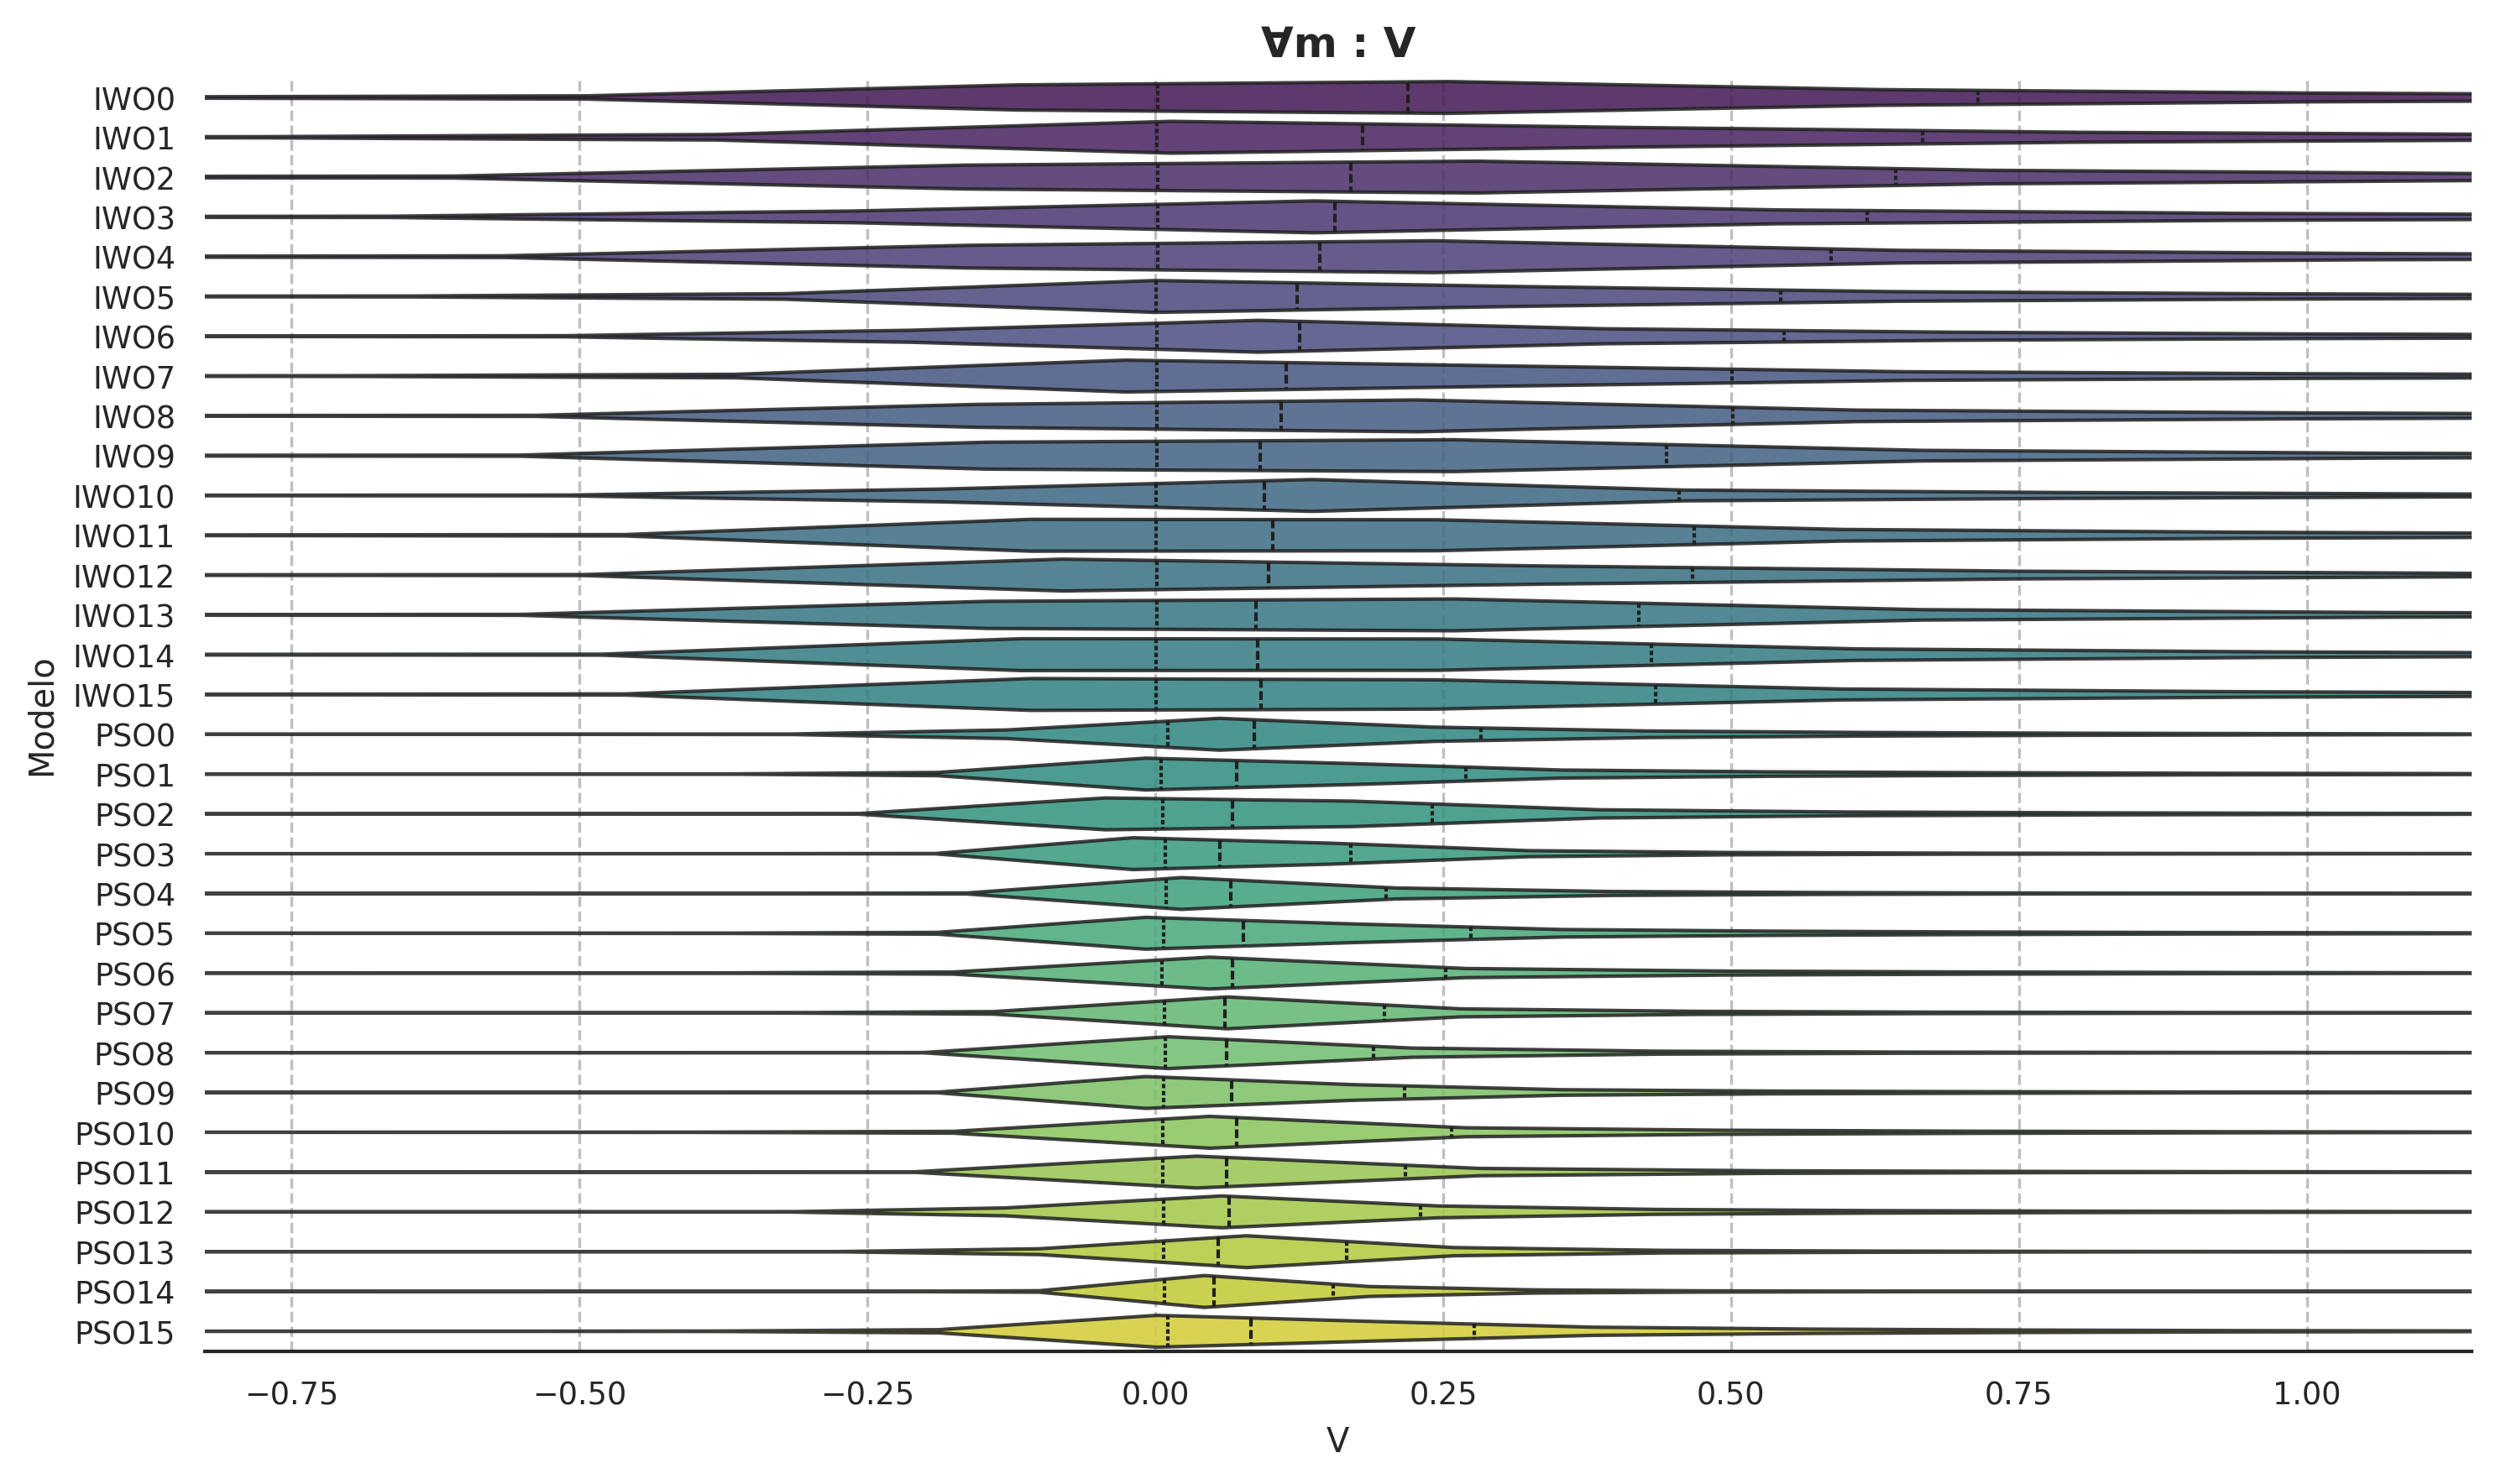
\includegraphics[width=\textwidth, height=0.65\textheight, keepaspectratio]{./plot_for_∀m_V.png}
      \caption{\small Comparativa distribuciones.}
    \end{figure}
  \end{columns}
\end{frame}

\begin{frame}{4. Experimento 2: Criterios Estadísticos y Conteo de Borda}
  \begin{columns}
    \column{0.52\textwidth}
    \begin{block}{Momentos Estadísticos}
      \begin{itemize}
        \item \textbf{\(s_1\):} Media de \(V_{\text{eff}}\).
        \item \textbf{\(s_2\):} Asimetría (\textit{Skewness}) de \(V_{\text{eff}}\).
        \item \textbf{\(s_3\):} Curtosis en la cola positiva de \(V_{\text{eff}}\).
        \item \textbf{\(s_4\):} Curtosis en la cola negativa de \(V_{\text{eff}}\).
        \item \textbf{\(s_5\):} Proporción de configuraciones estables.
        \item \textbf{\(s_6\):} Proporción de vacíos estables de Sitter (\(dS\)).
        \item \textbf{\(s_7\):} Límites de convergencia de la aptitud.
      \end{itemize}
    \end{block}

    \column{0.48\textwidth}
    \begin{alertblock}{Conteo de Borda}
      Asignación posicional (\(n-1\) puntos al mejor y $0$ al peor en cada criterio \(j\)):
      
      \begin{equation*}
        B_i = \sum_{j} P_{ij}, \quad i \in \{0, \dots, n-1\}
      \end{equation*}
      
      donde \(B_i\) es el índice global del optimizador \(i\).
    \end{alertblock}
  \end{columns}
\end{frame}

\begin{frame}{4. Experimento 2: Criterios Estadísticos y Conteo de Borda}
    \begin{figure}
      \centering
      % Reemplaza con la ruta de tu gráfica para el Exp 2
      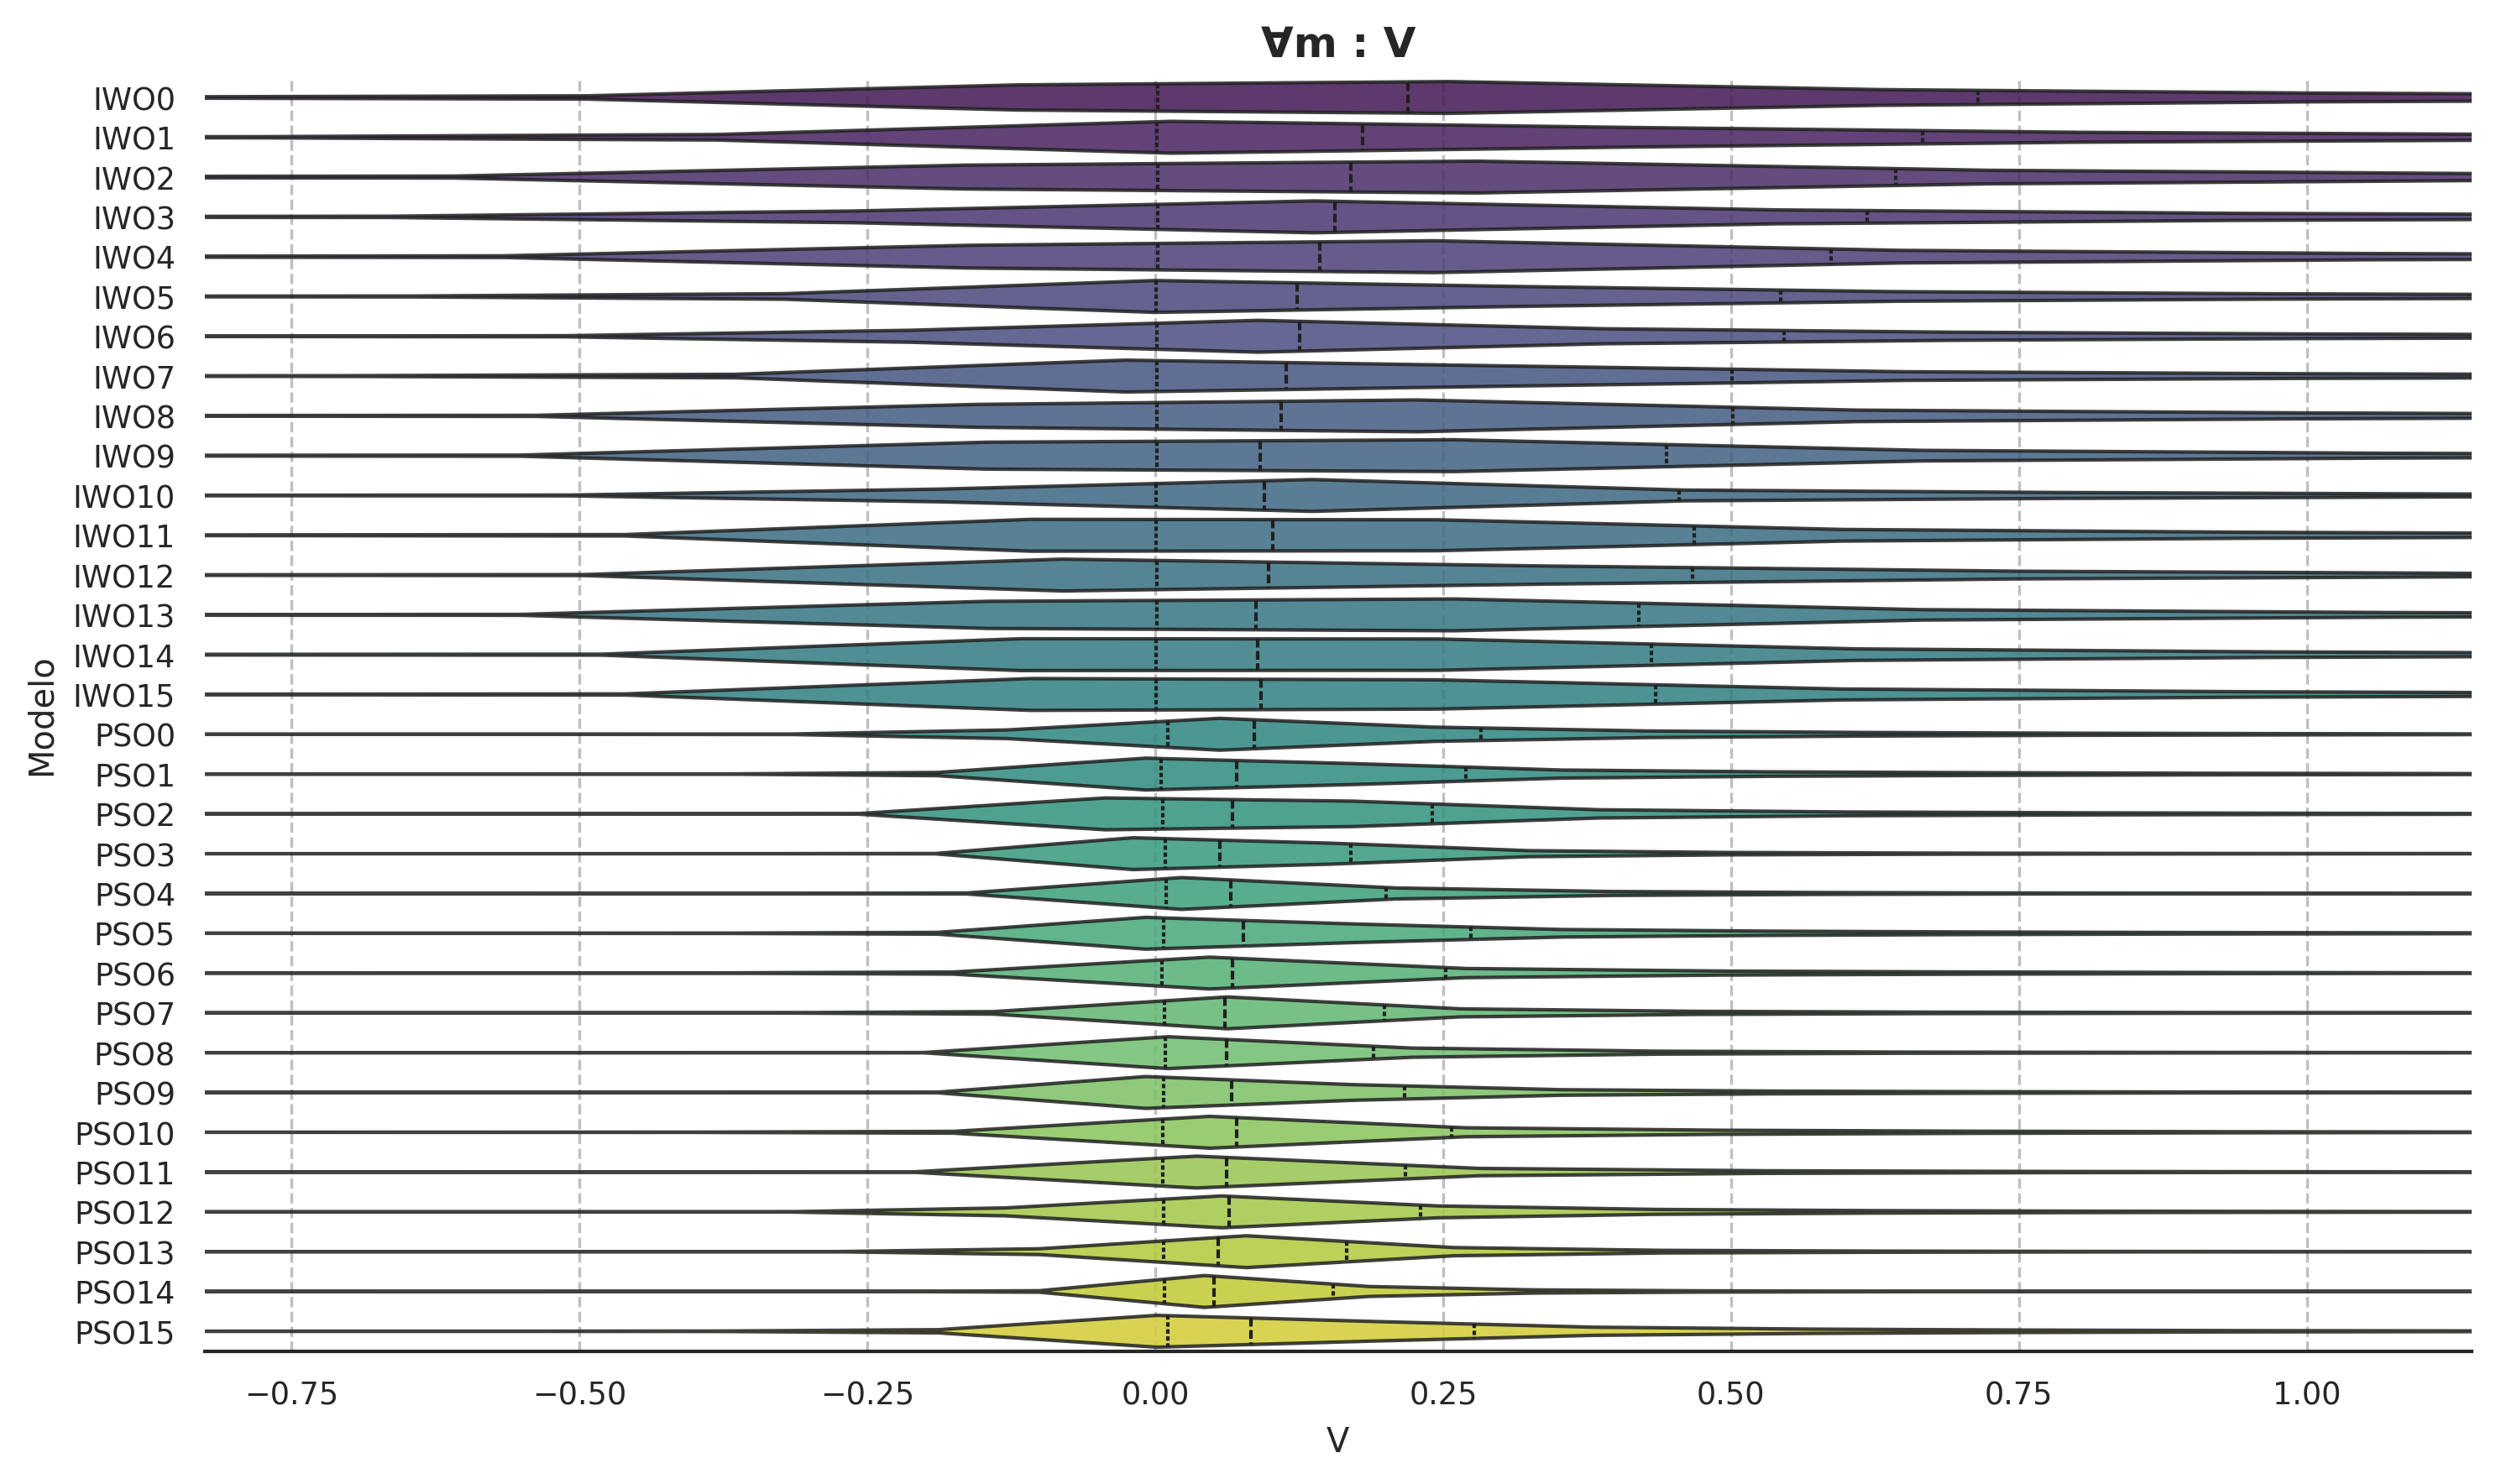
\includegraphics[width=\textwidth, height=0.65\textheight, keepaspectratio]{./plot_for_∀m_V.png}
      \caption{\small Comparativa de mejores metaheurísticos.}
    \end{figure}
\end{frame}

\begin{frame}{5. Experimento 3: Reducción de Dimensionalidad y Clasificación}
  \begin{columns}
    \column{0.48\textwidth}
    \begin{block}{Metodología y Agrupamiento}
      Para caracterizar el paisaje de mínimos identificado, se aplicaron técnicas de aprendizaje no supervisado y reducción de dimensionalidad sobre el espacio de características.

      \vspace{0.2cm}

      Mediante análisis de componentes principales (PCA) y algoritmos de aglomeración, se mapeó la topología de los vacíos para clasificar familias de soluciones según su estabilidad física.
    \end{block}

    \column{0.52\textwidth}
    \begin{figure}
      \centering
      % Reemplaza con la ruta de tu gráfica para el Exp 3
      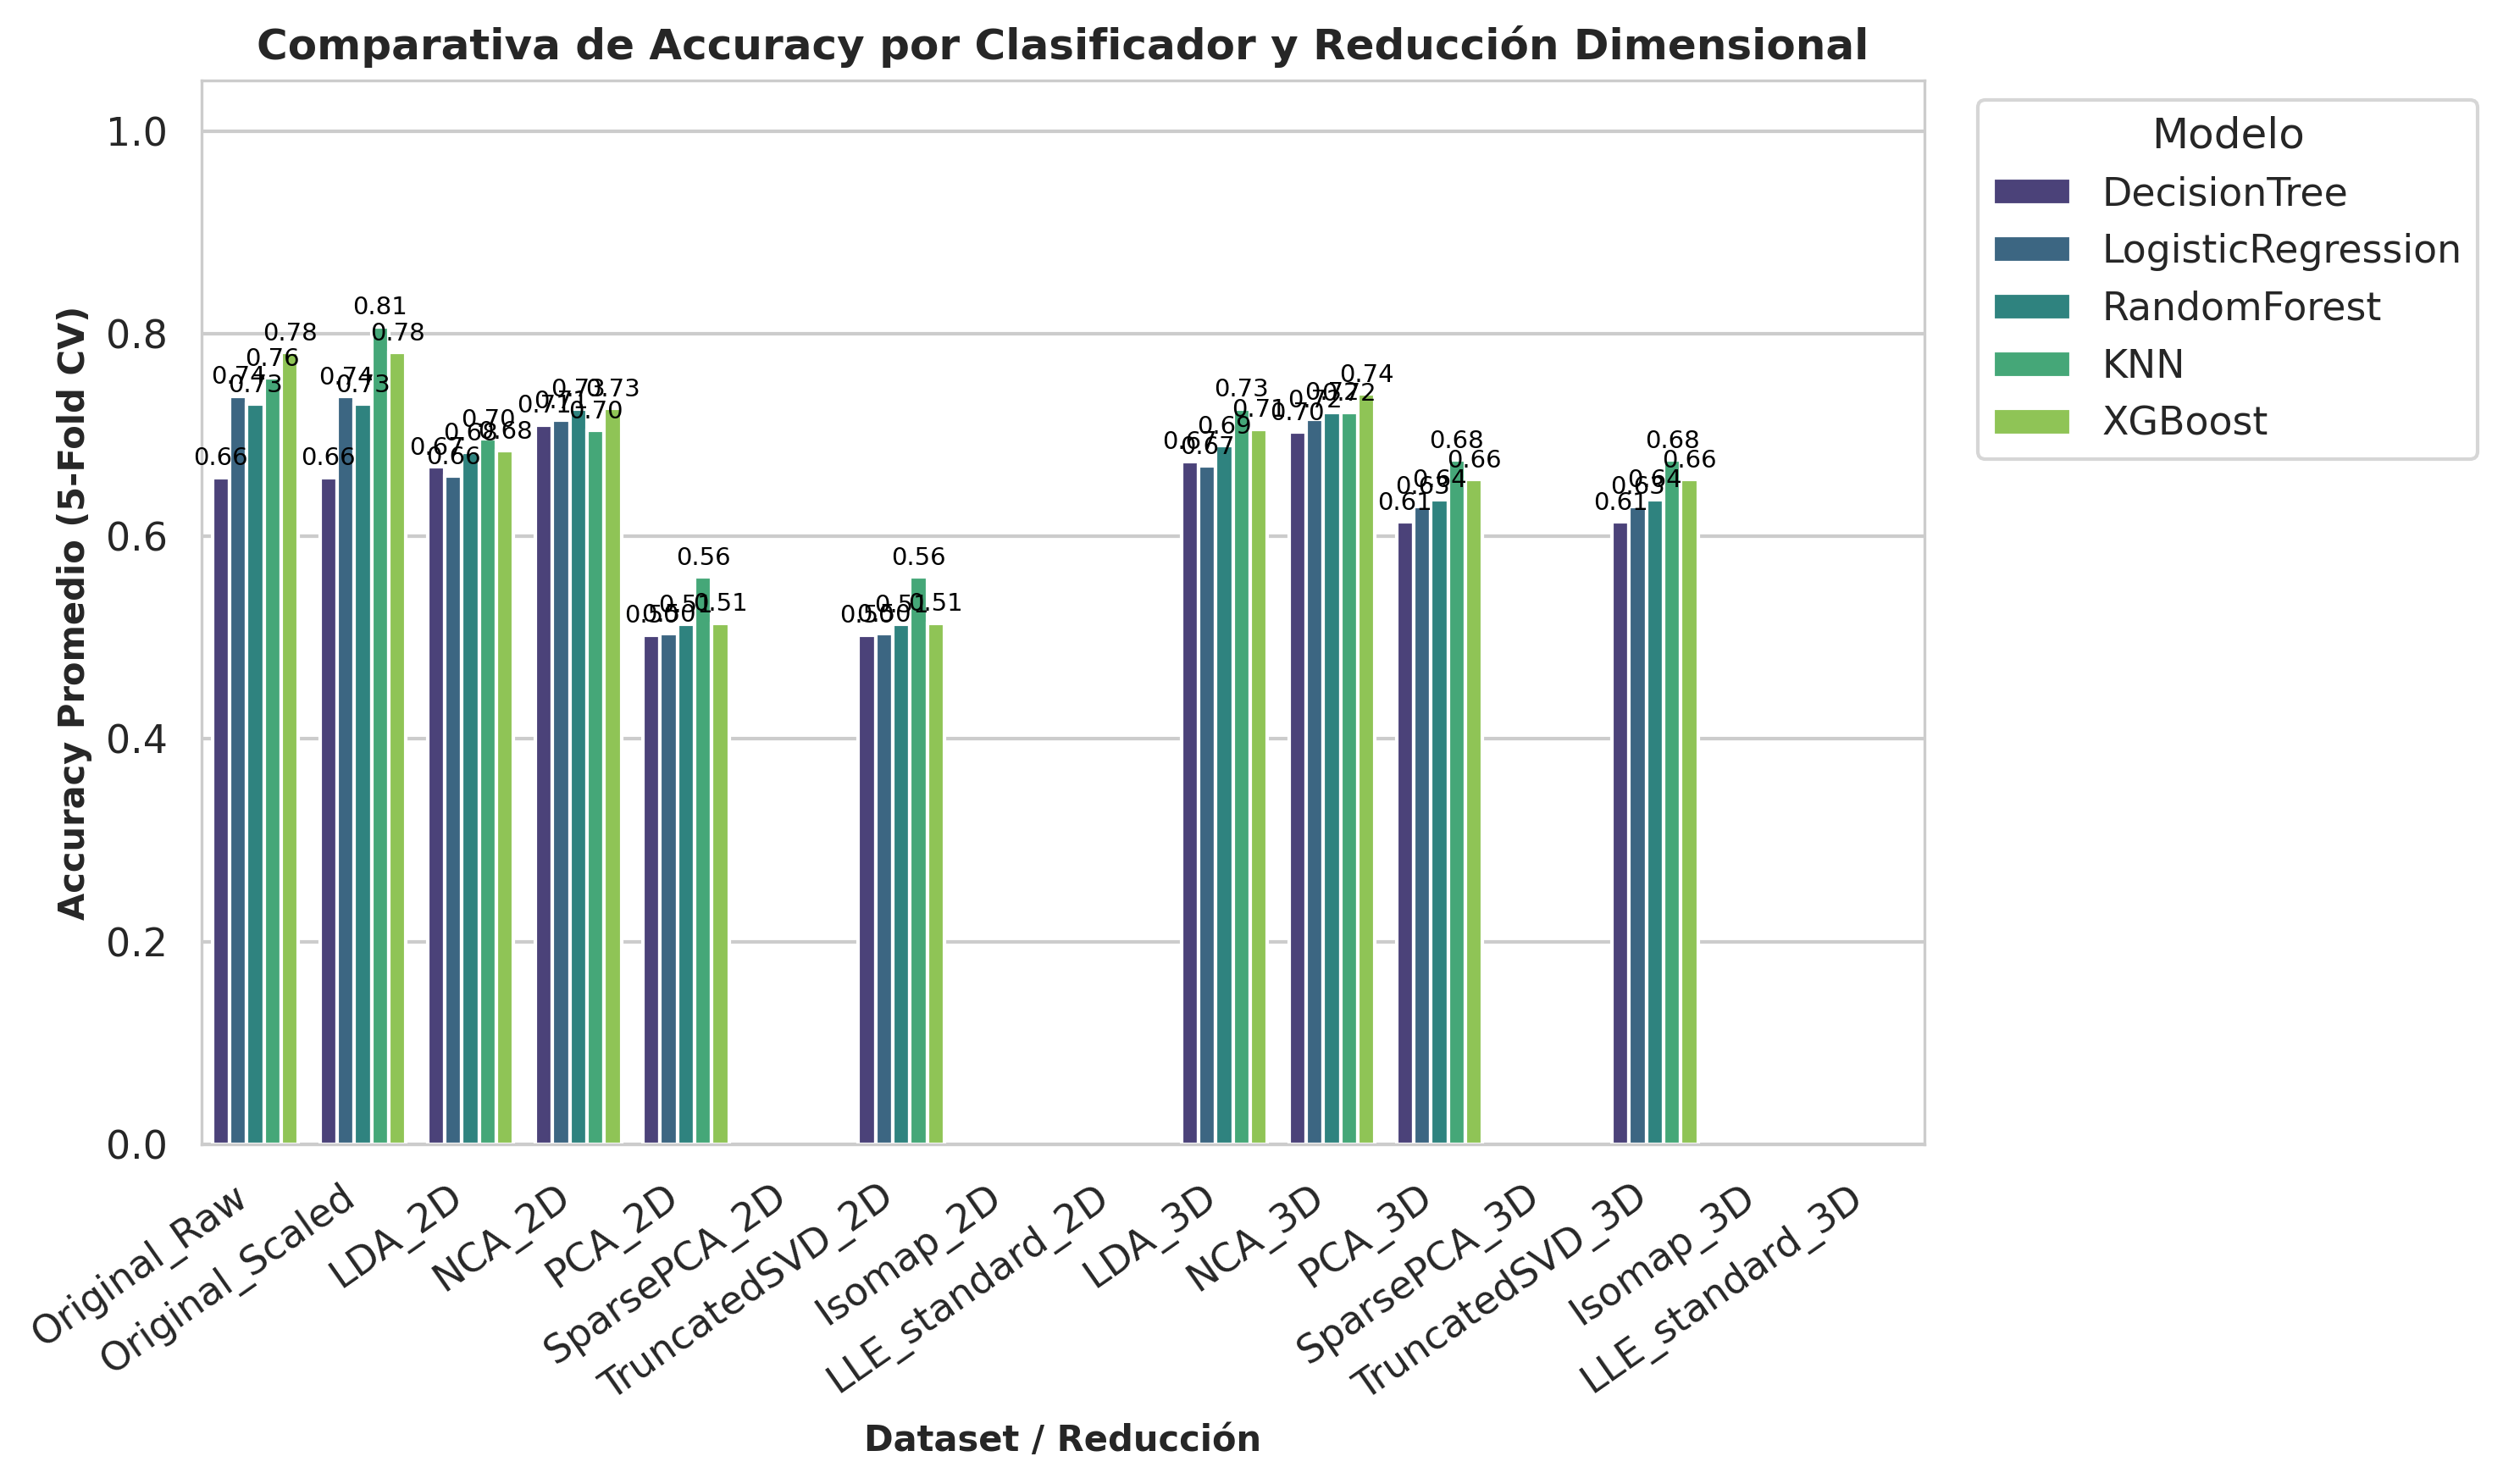
\includegraphics[width=\textwidth, height=0.65\textheight, keepaspectratio]{./HIST_COMPARATIVE_DIMRED_CLASS.png}
      \caption{\small Preliminar, rendimiento de clasificadores.}
    \end{figure}
  \end{columns}
\end{frame}

% --- Isomap ---
\begin{frame}{Experimento 3: Reducción de Dimensionalidad — Isomap}
  \begin{columns}
    \column{0.50\textwidth}
    \begin{figure}
      \centering
      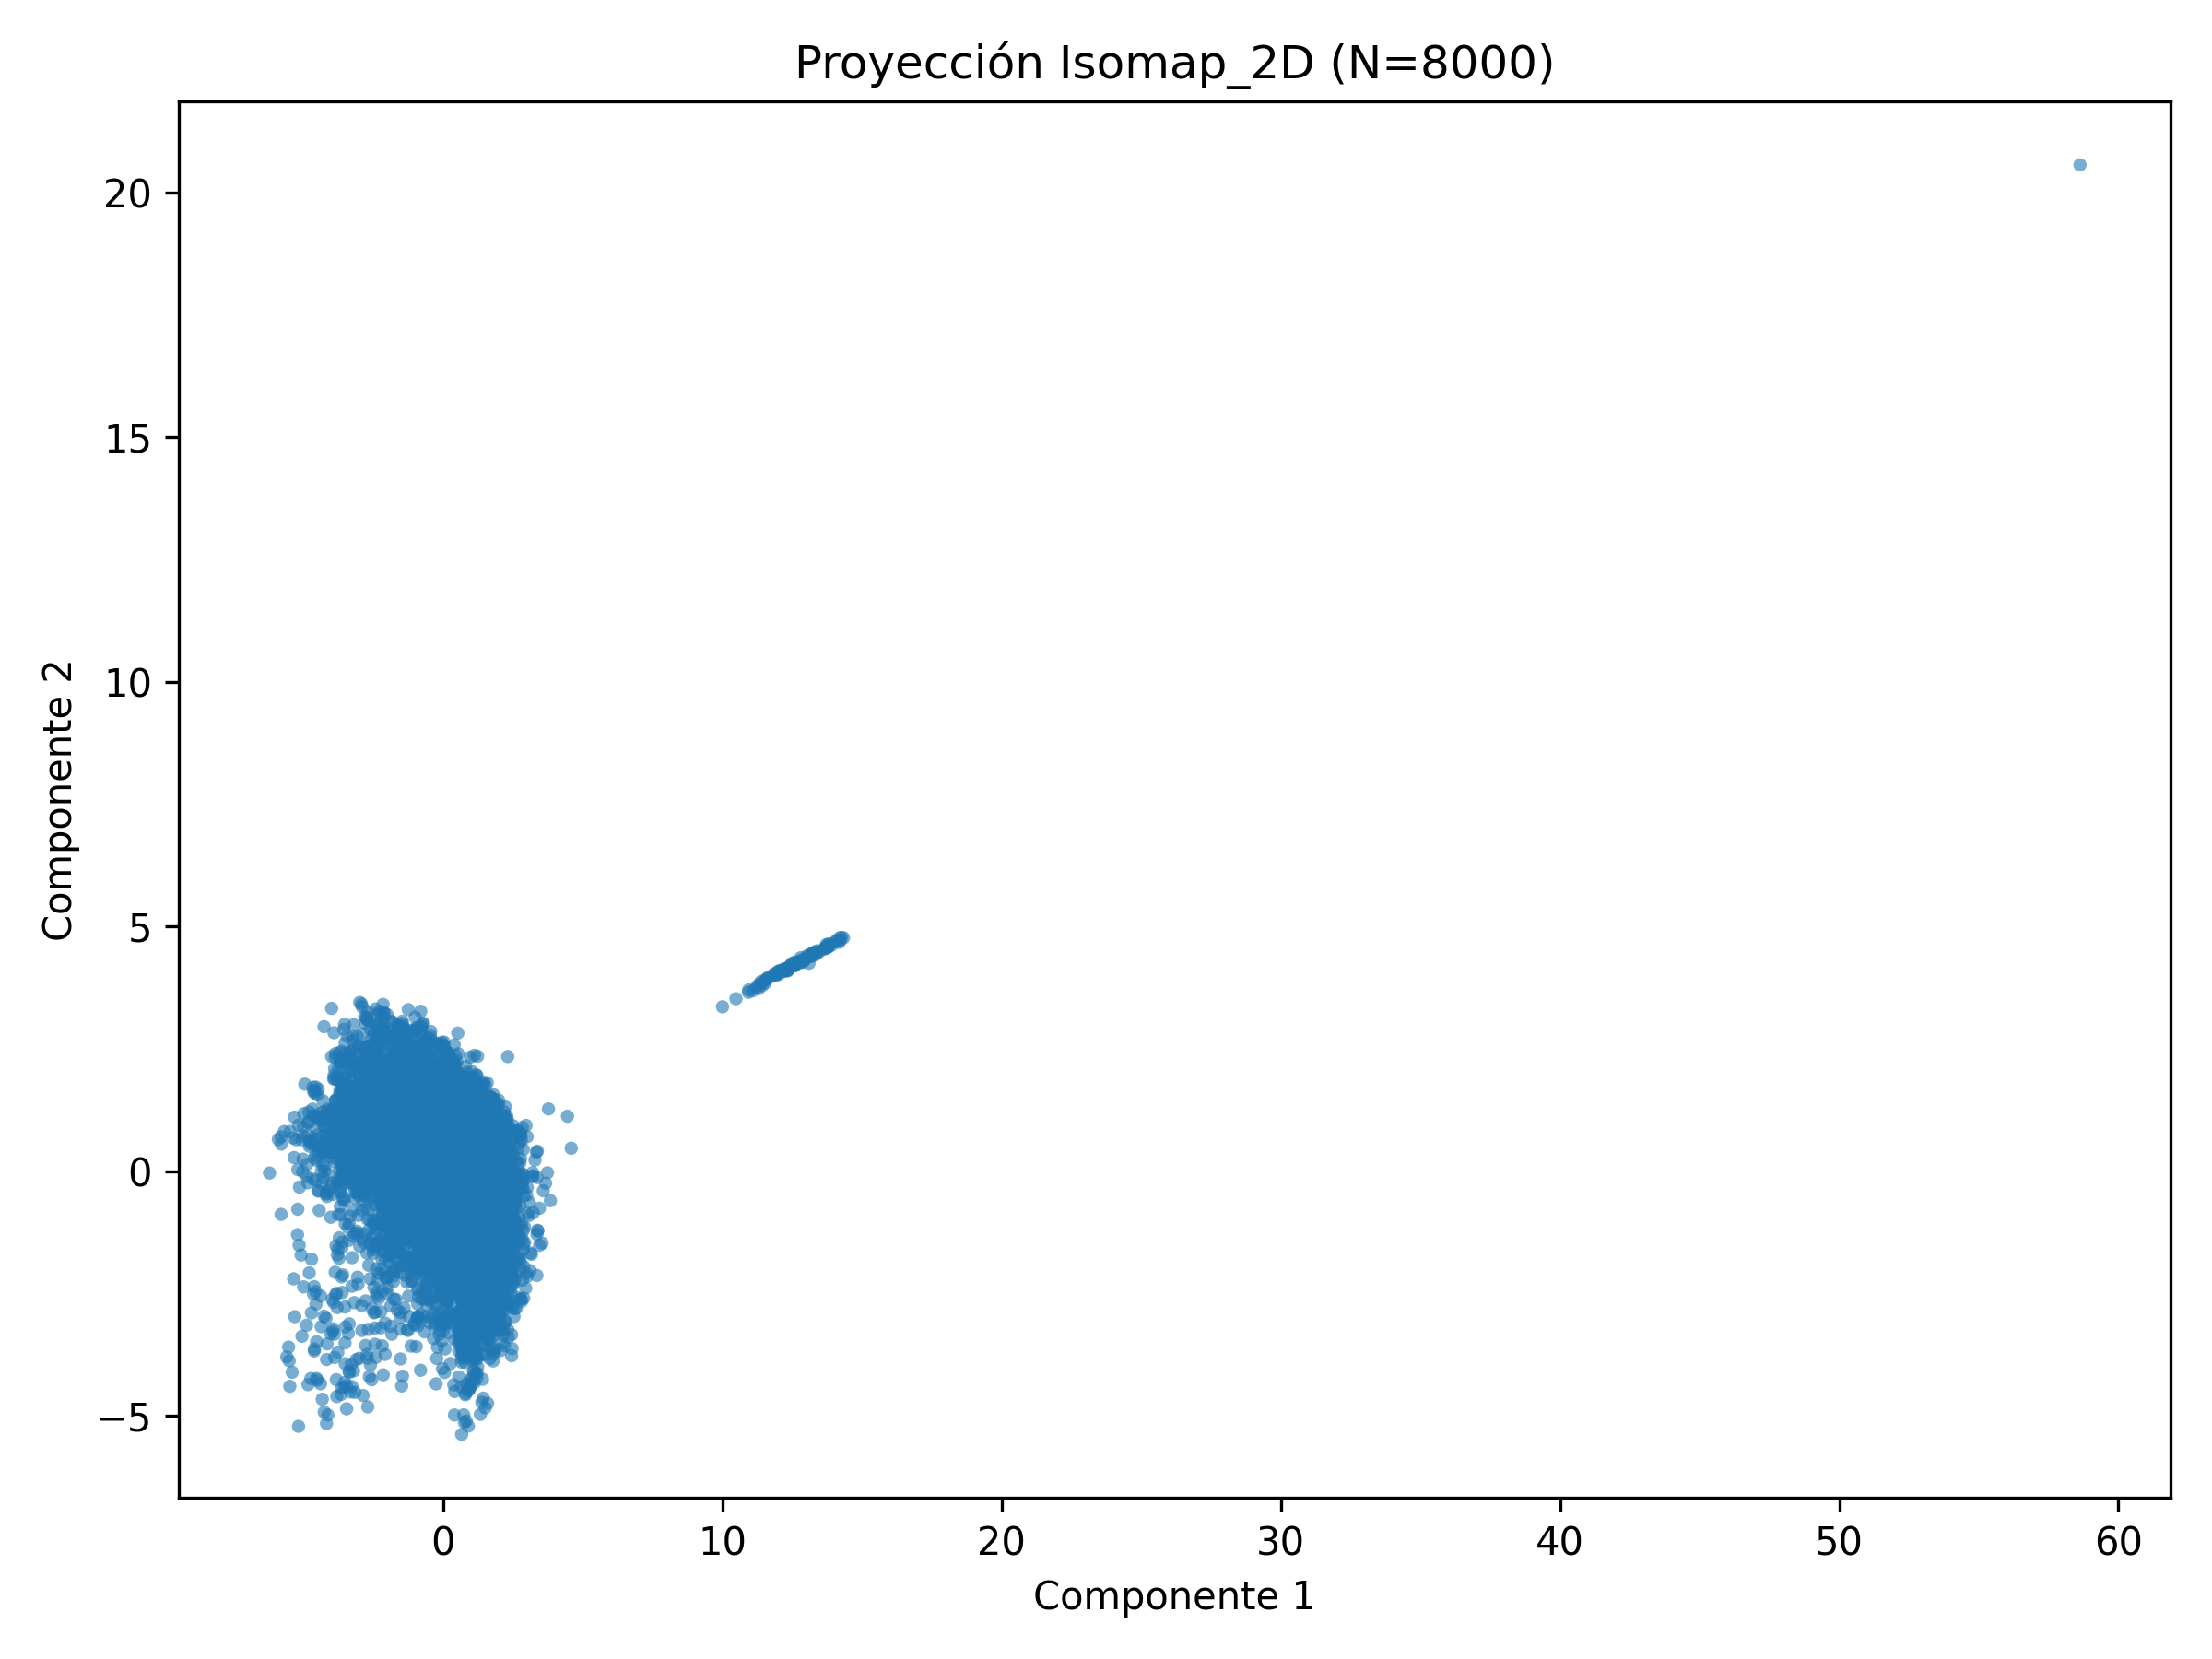
\includegraphics[width=\textwidth, height=0.75\textheight, keepaspectratio]{plot_Isomap_2D.png}
      \caption{\small Proyección Isomap 2D}
    \end{figure}
    
    \column{0.50\textwidth}
    \begin{figure}
      \centering
      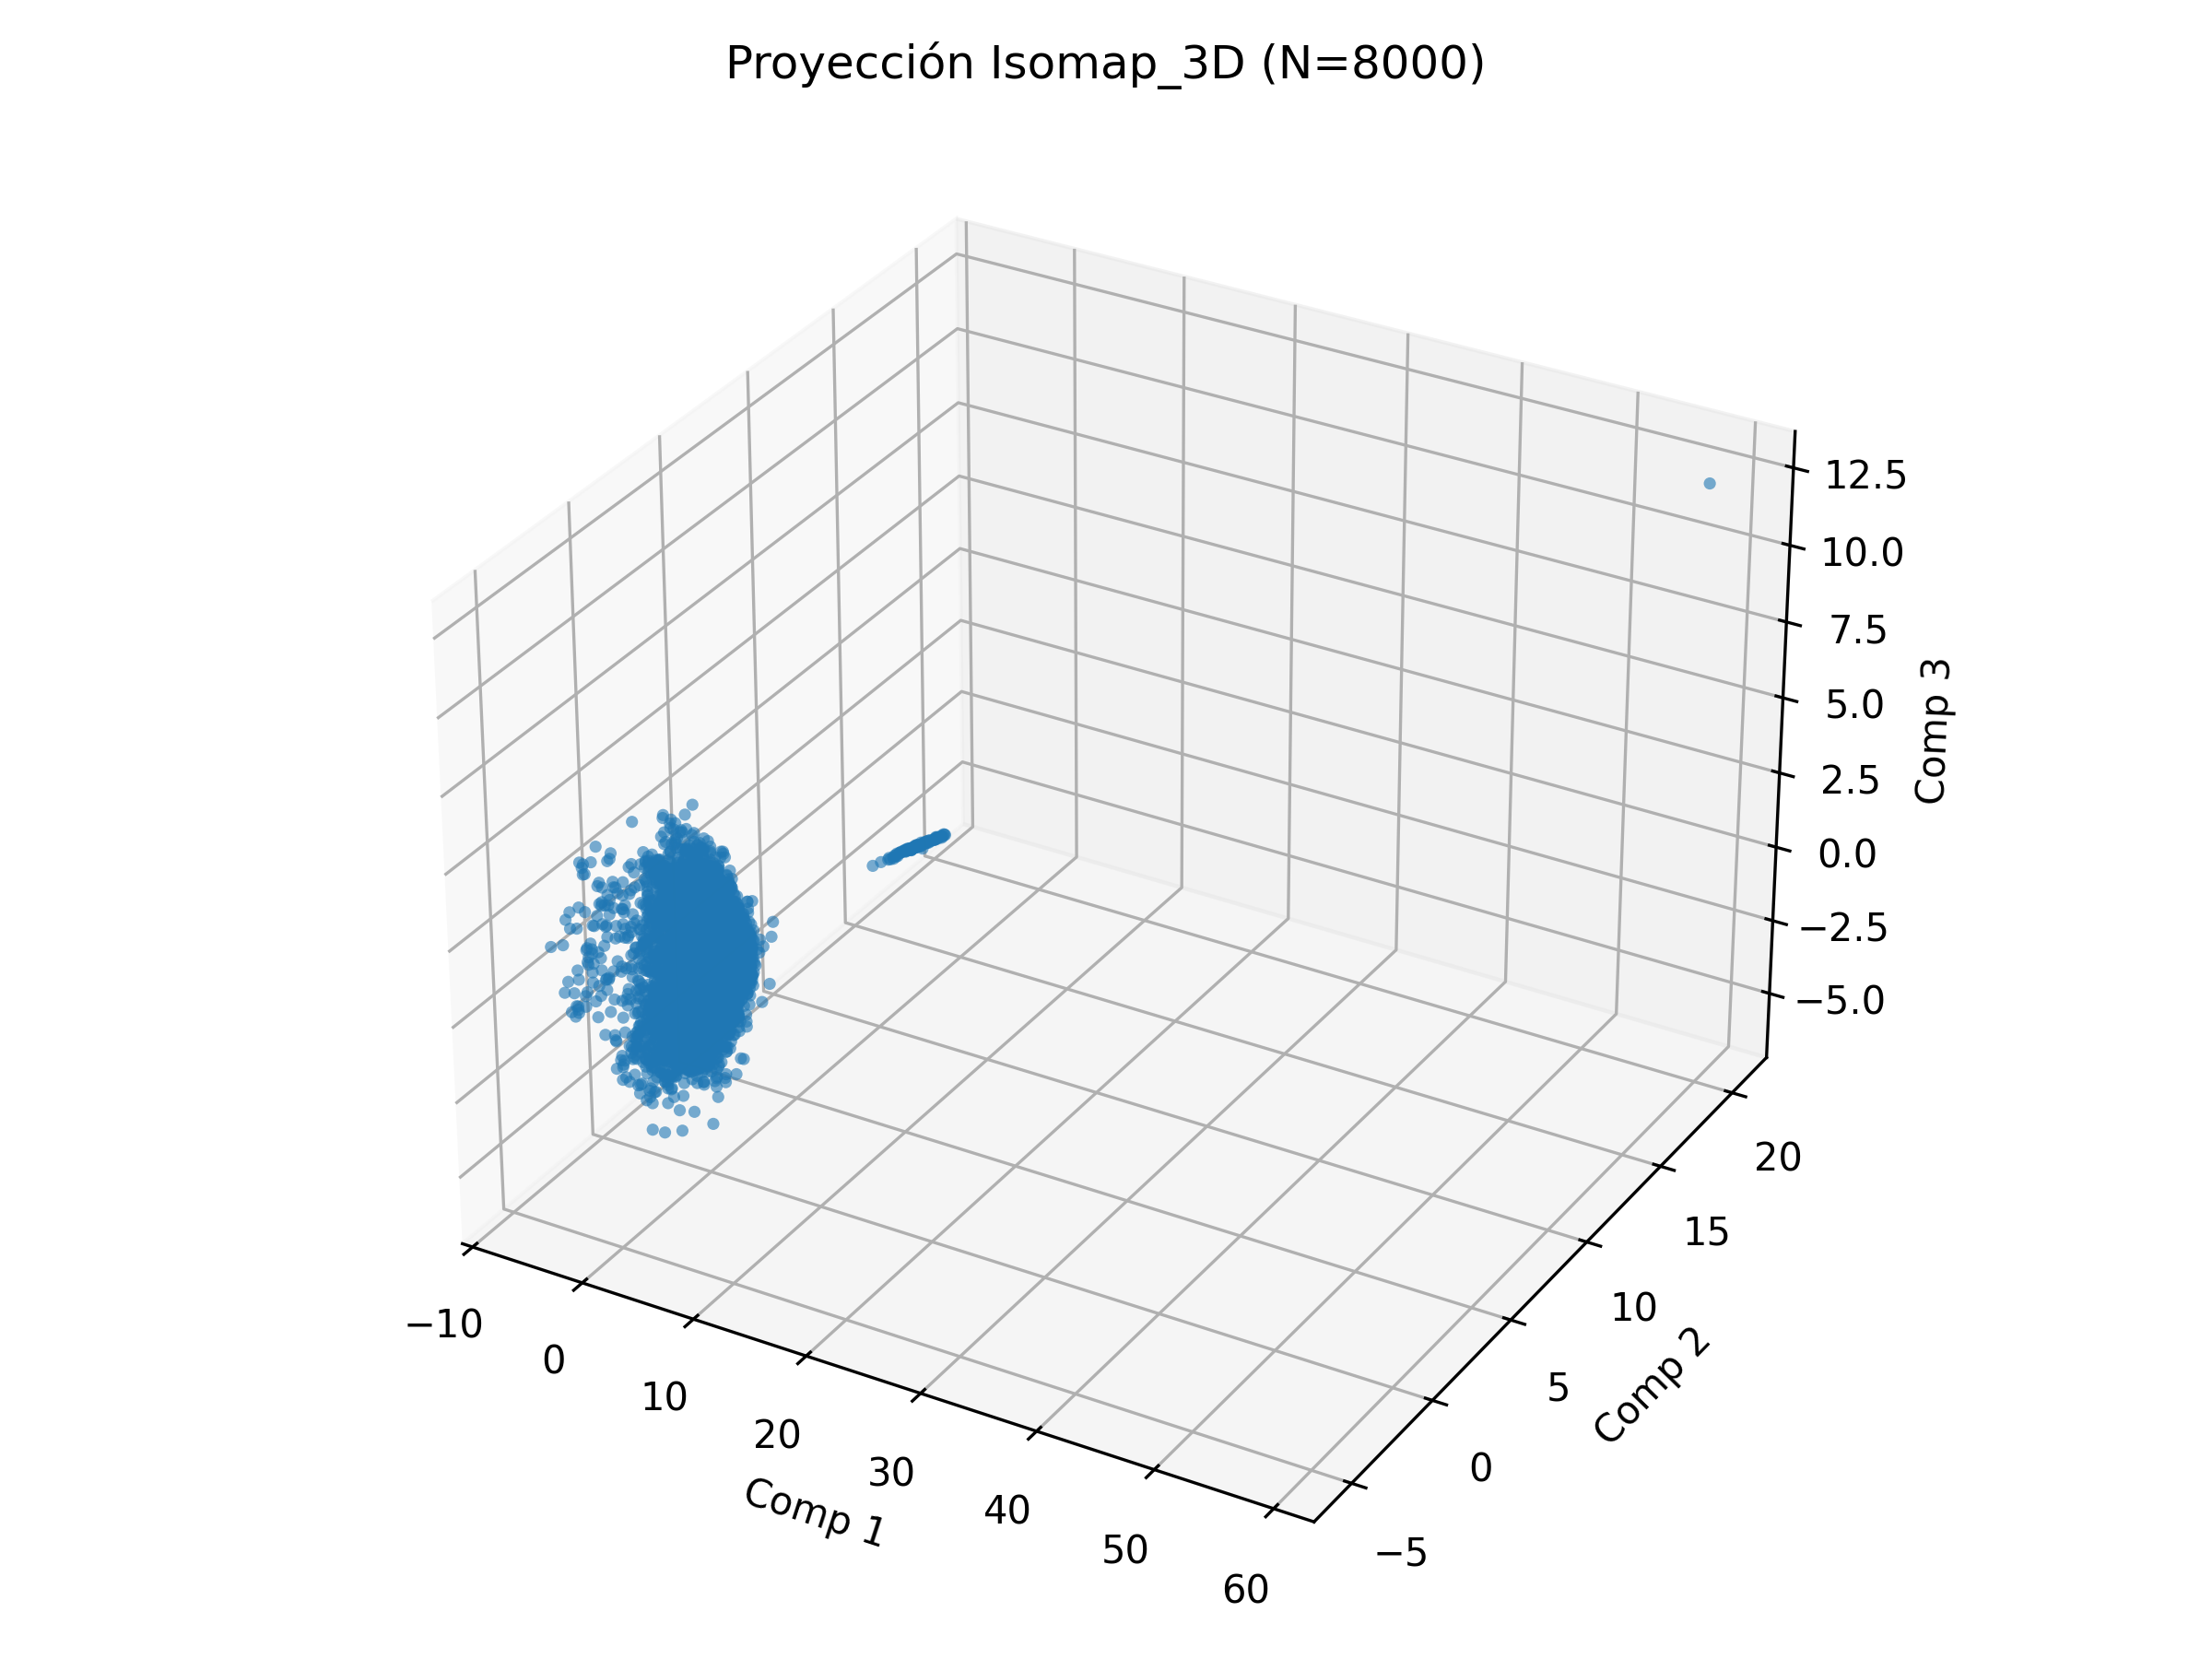
\includegraphics[width=\textwidth, height=0.75\textheight, keepaspectratio]{plot_Isomap_3D.png}
      \caption{\small Proyección Isomap 3D}
    \end{figure}
  \end{columns}
\end{frame}

% --- LDA ---
\begin{frame}{Experimento 3: Reducción de Dimensionalidad — LDA}
  \begin{columns}
    \column{0.50\textwidth}
    \begin{figure}
      \centering
      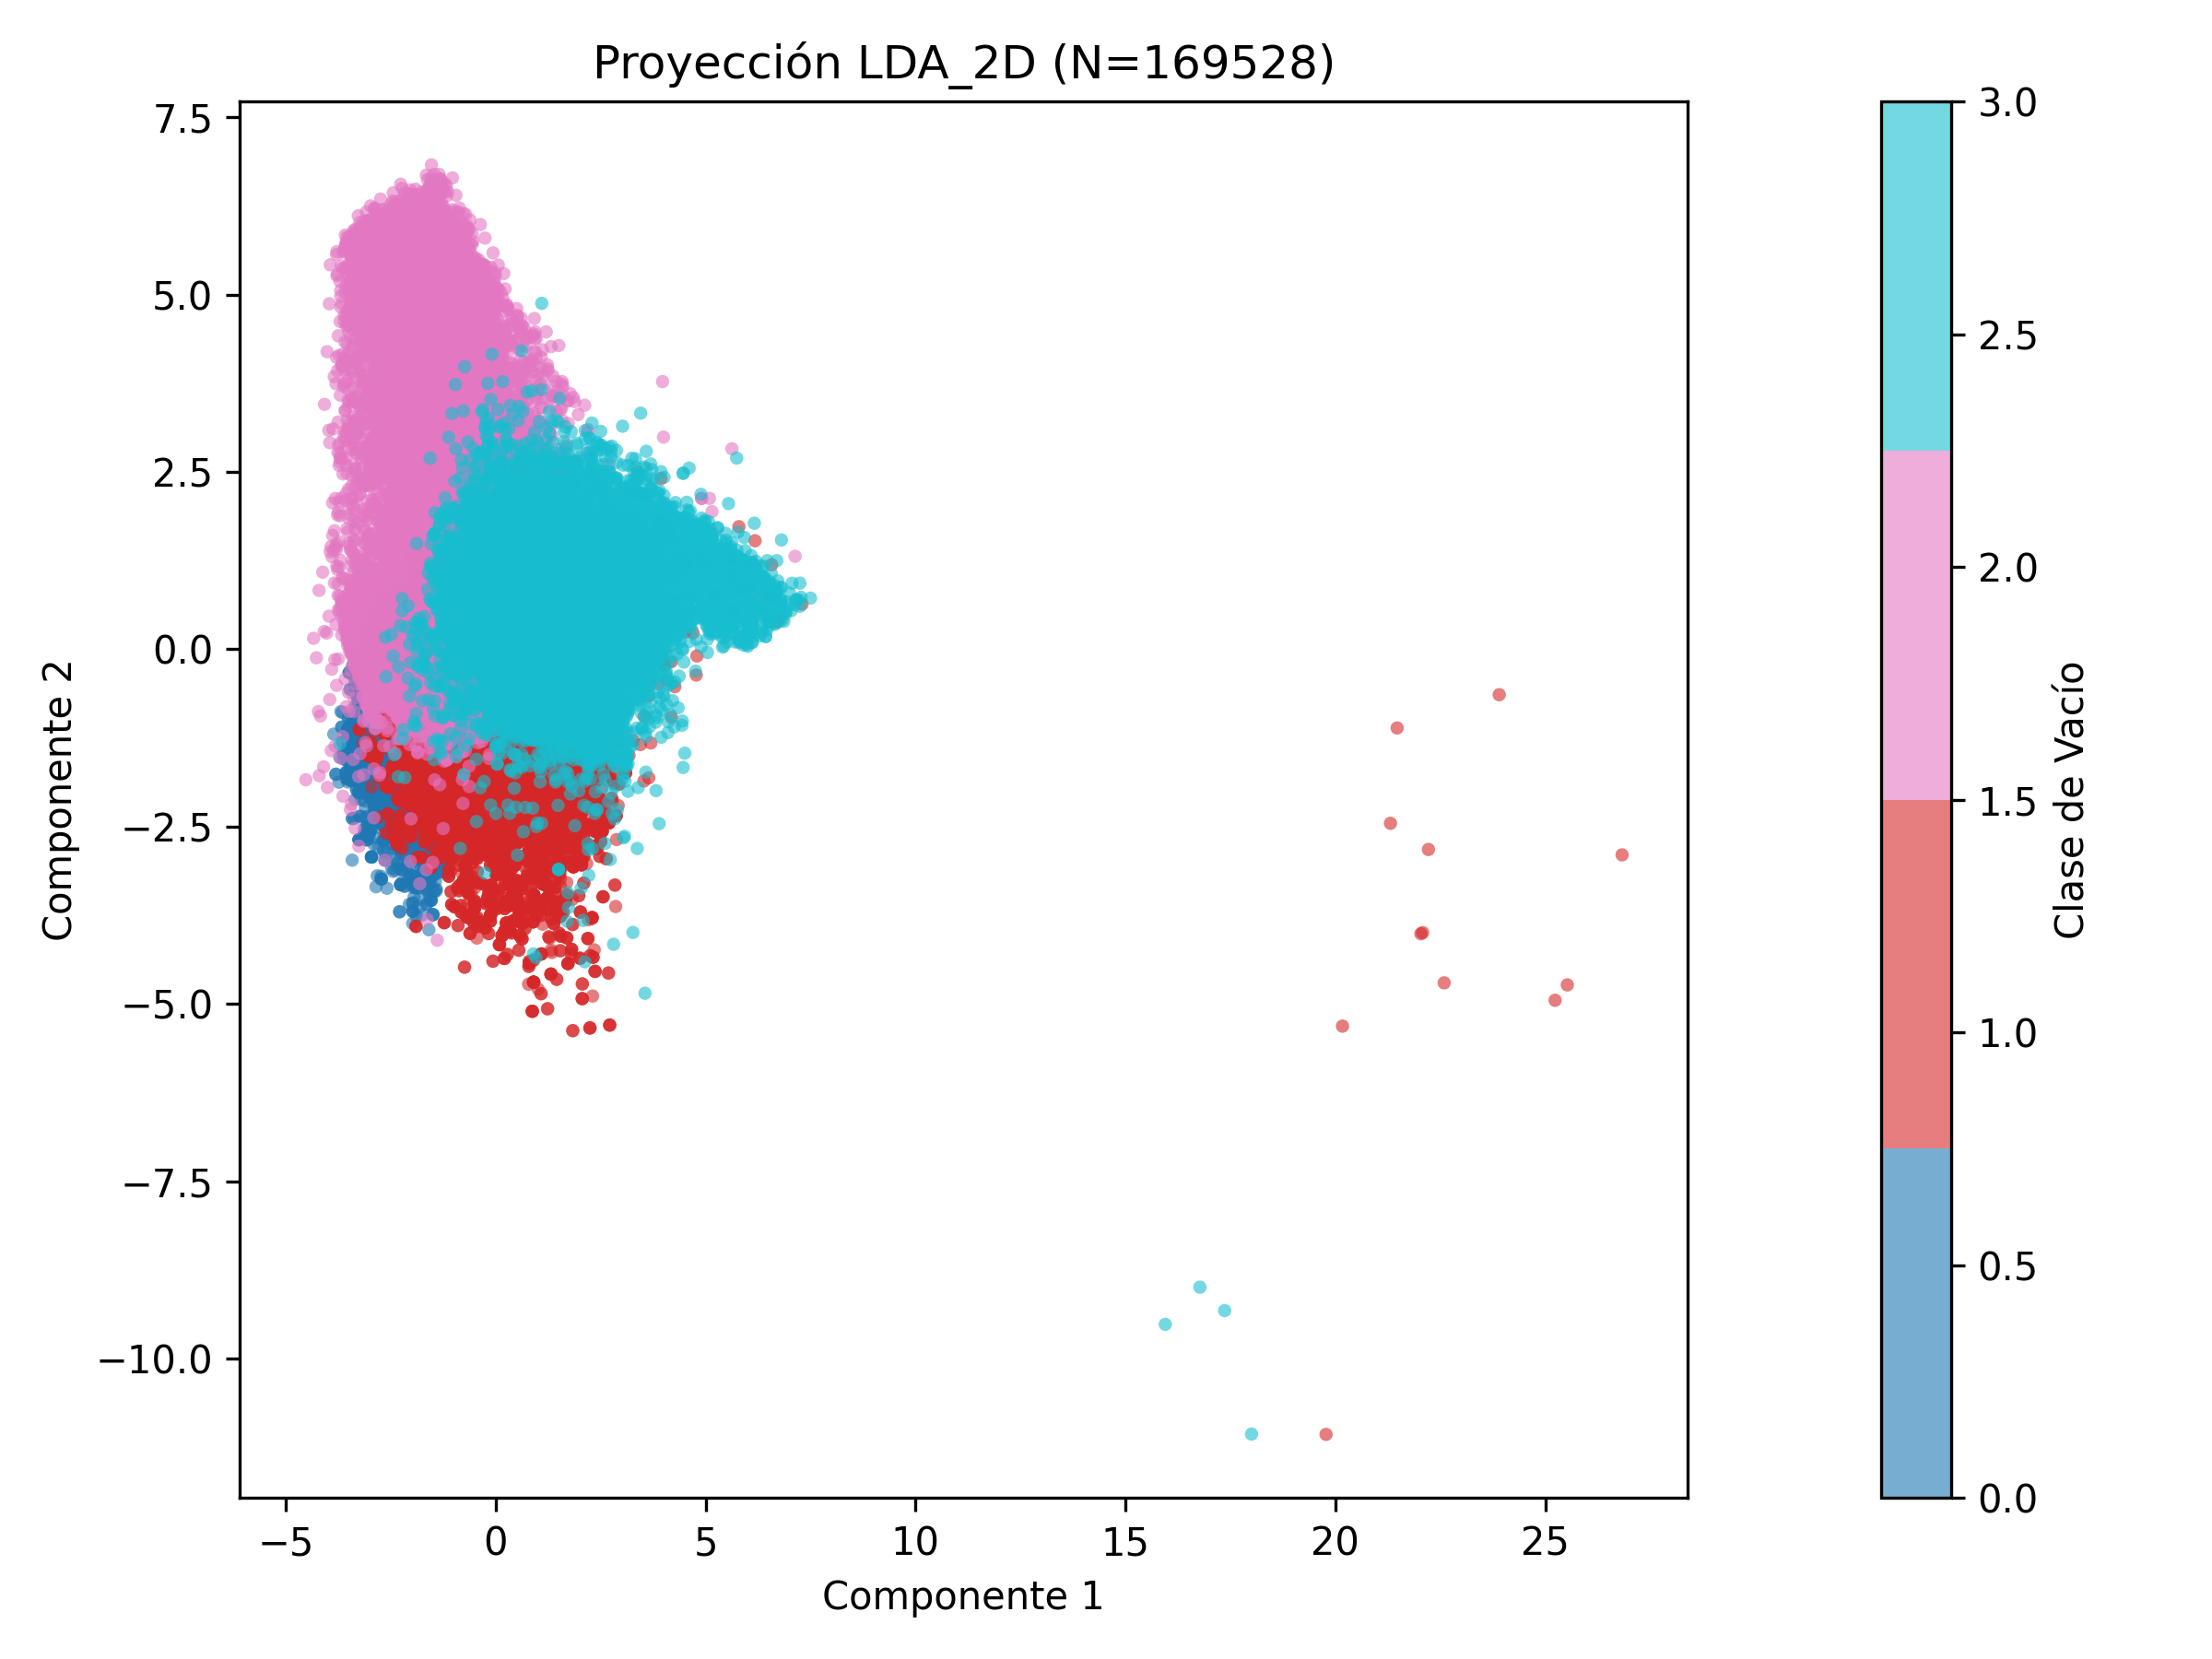
\includegraphics[width=\textwidth, height=0.75\textheight, keepaspectratio]{plot_LDA_2D.png}
      \caption{\small Proyección LDA 2D}
    \end{figure}
    
    \column{0.50\textwidth}
    \begin{figure}
      \centering
      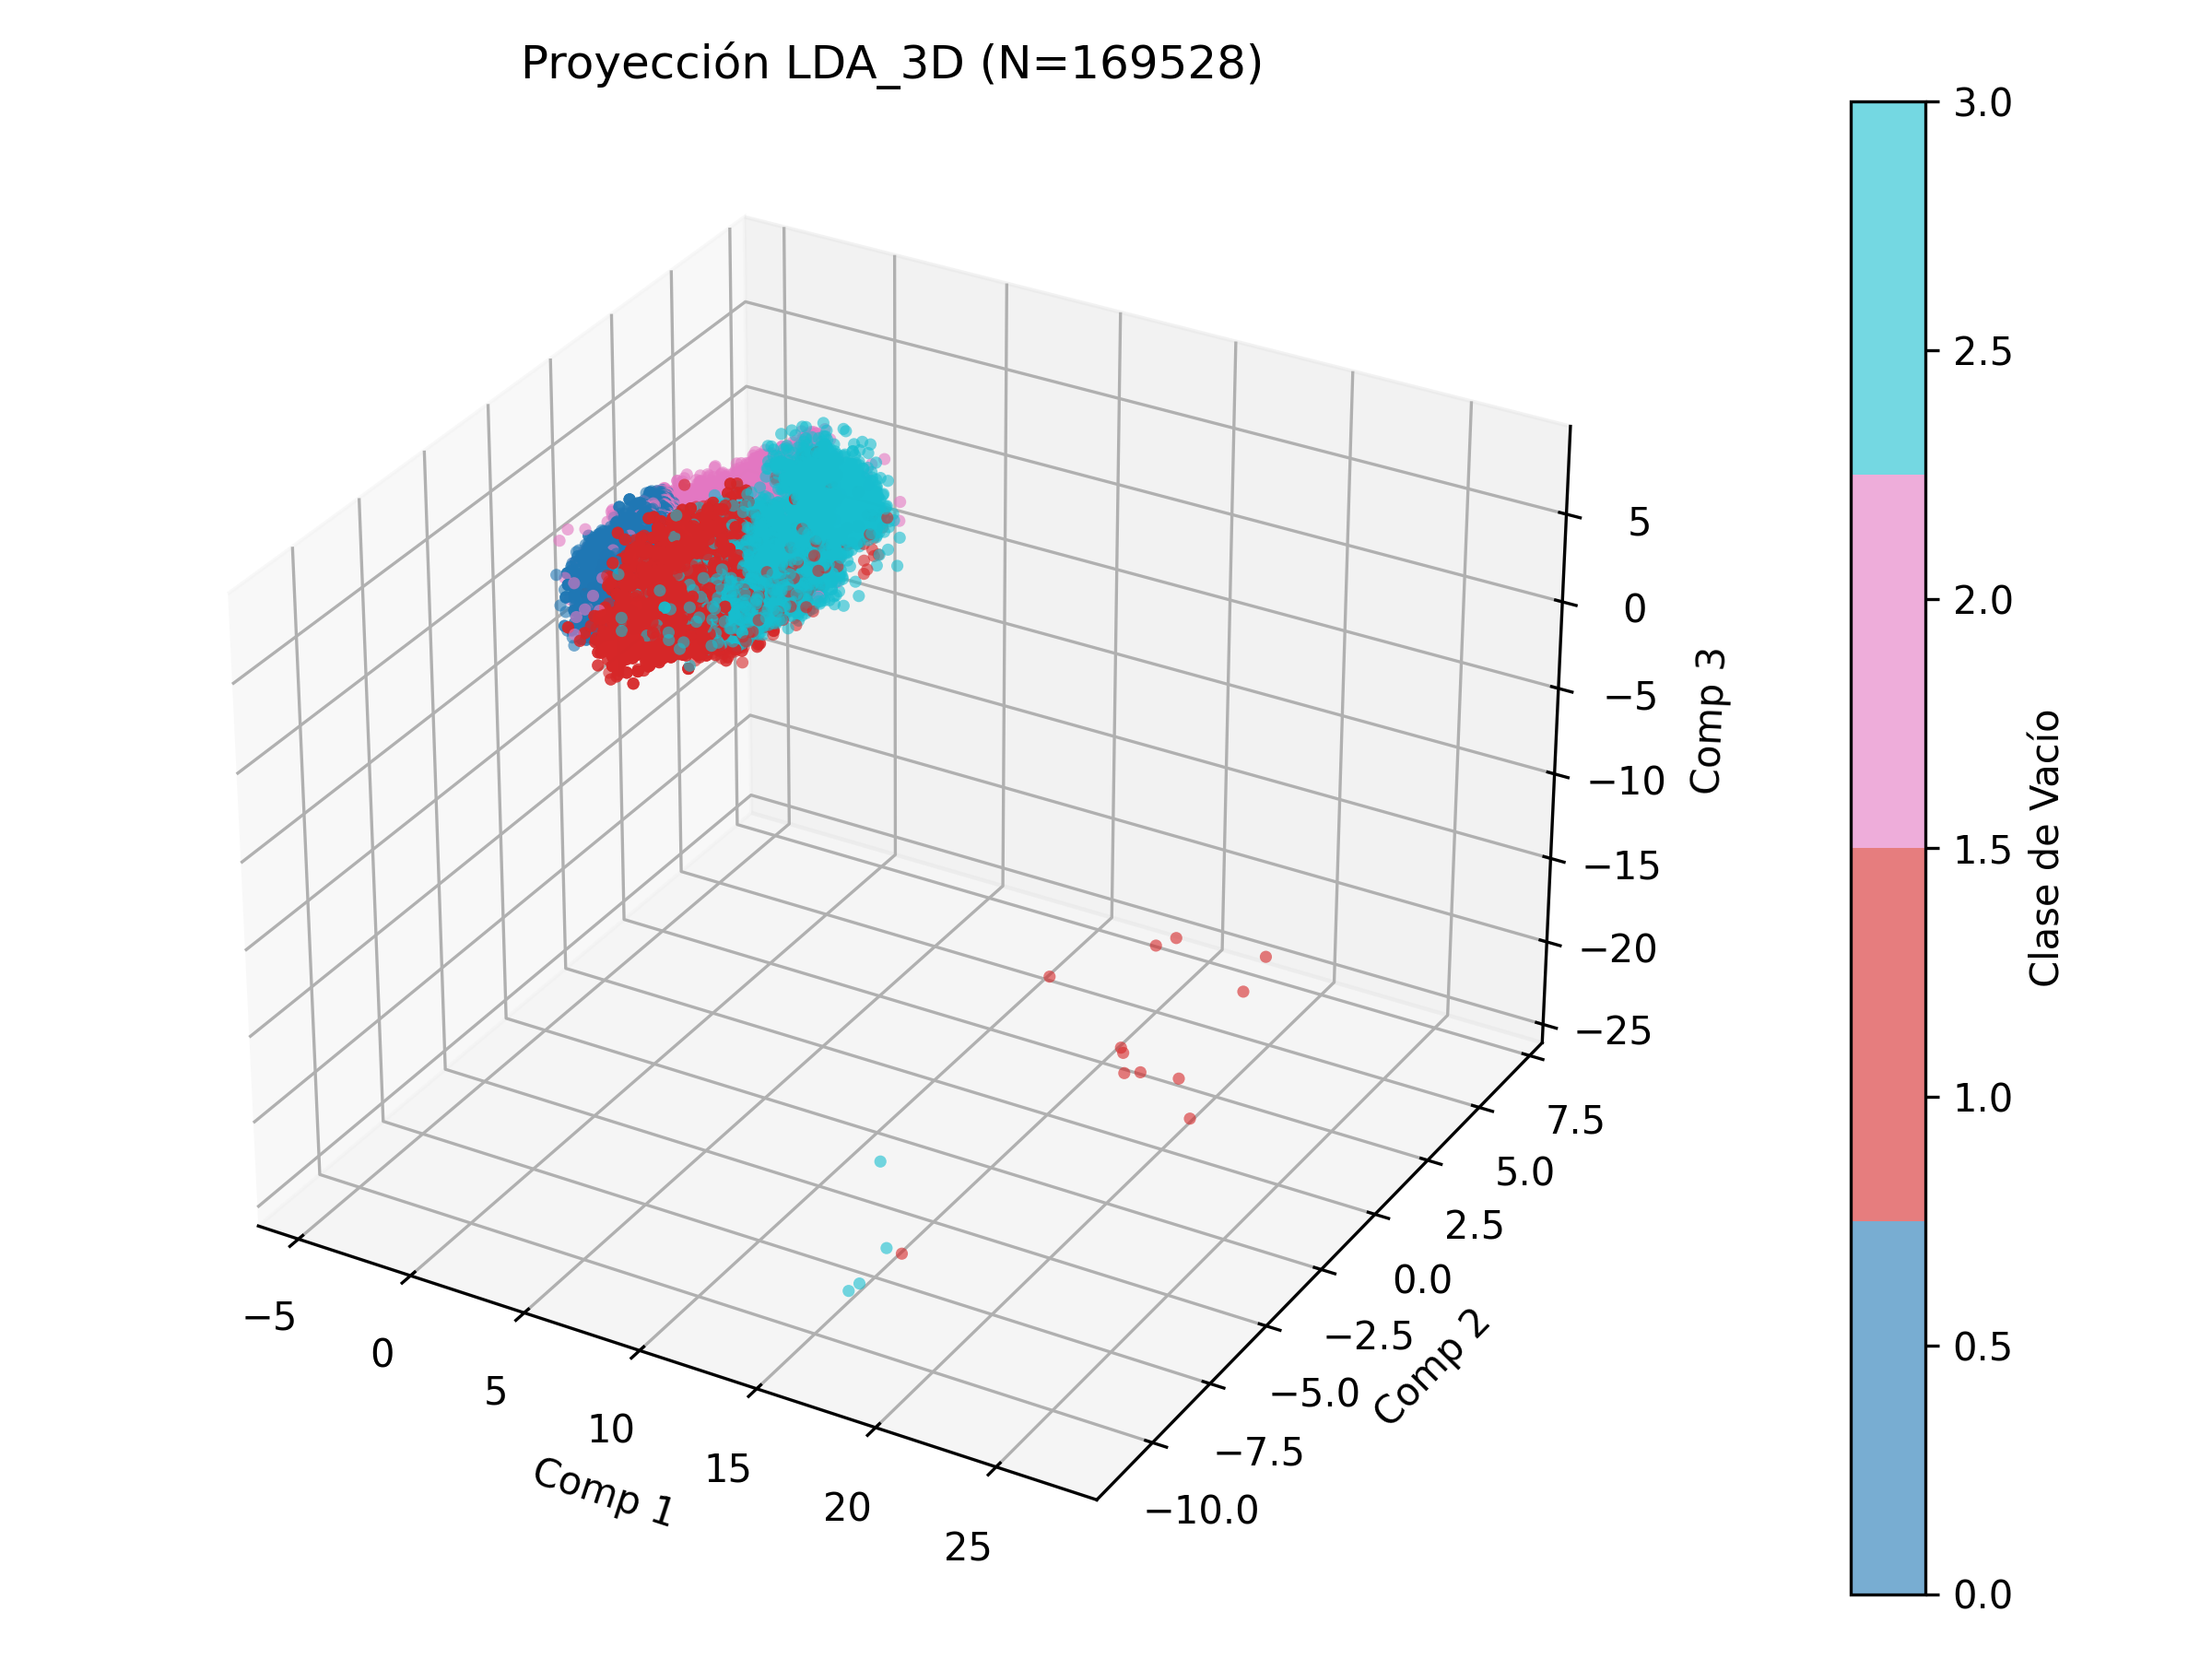
\includegraphics[width=\textwidth, height=0.75\textheight, keepaspectratio]{plot_LDA_3D.png}
      \caption{\small Proyección LDA 3D}
    \end{figure}
  \end{columns}
\end{frame}

% --- LLE ---
\begin{frame}{Experimento 3: Reducción de Dimensionalidad — LLE}
  \begin{columns}
    \column{0.50\textwidth}
    \begin{figure}
      \centering
      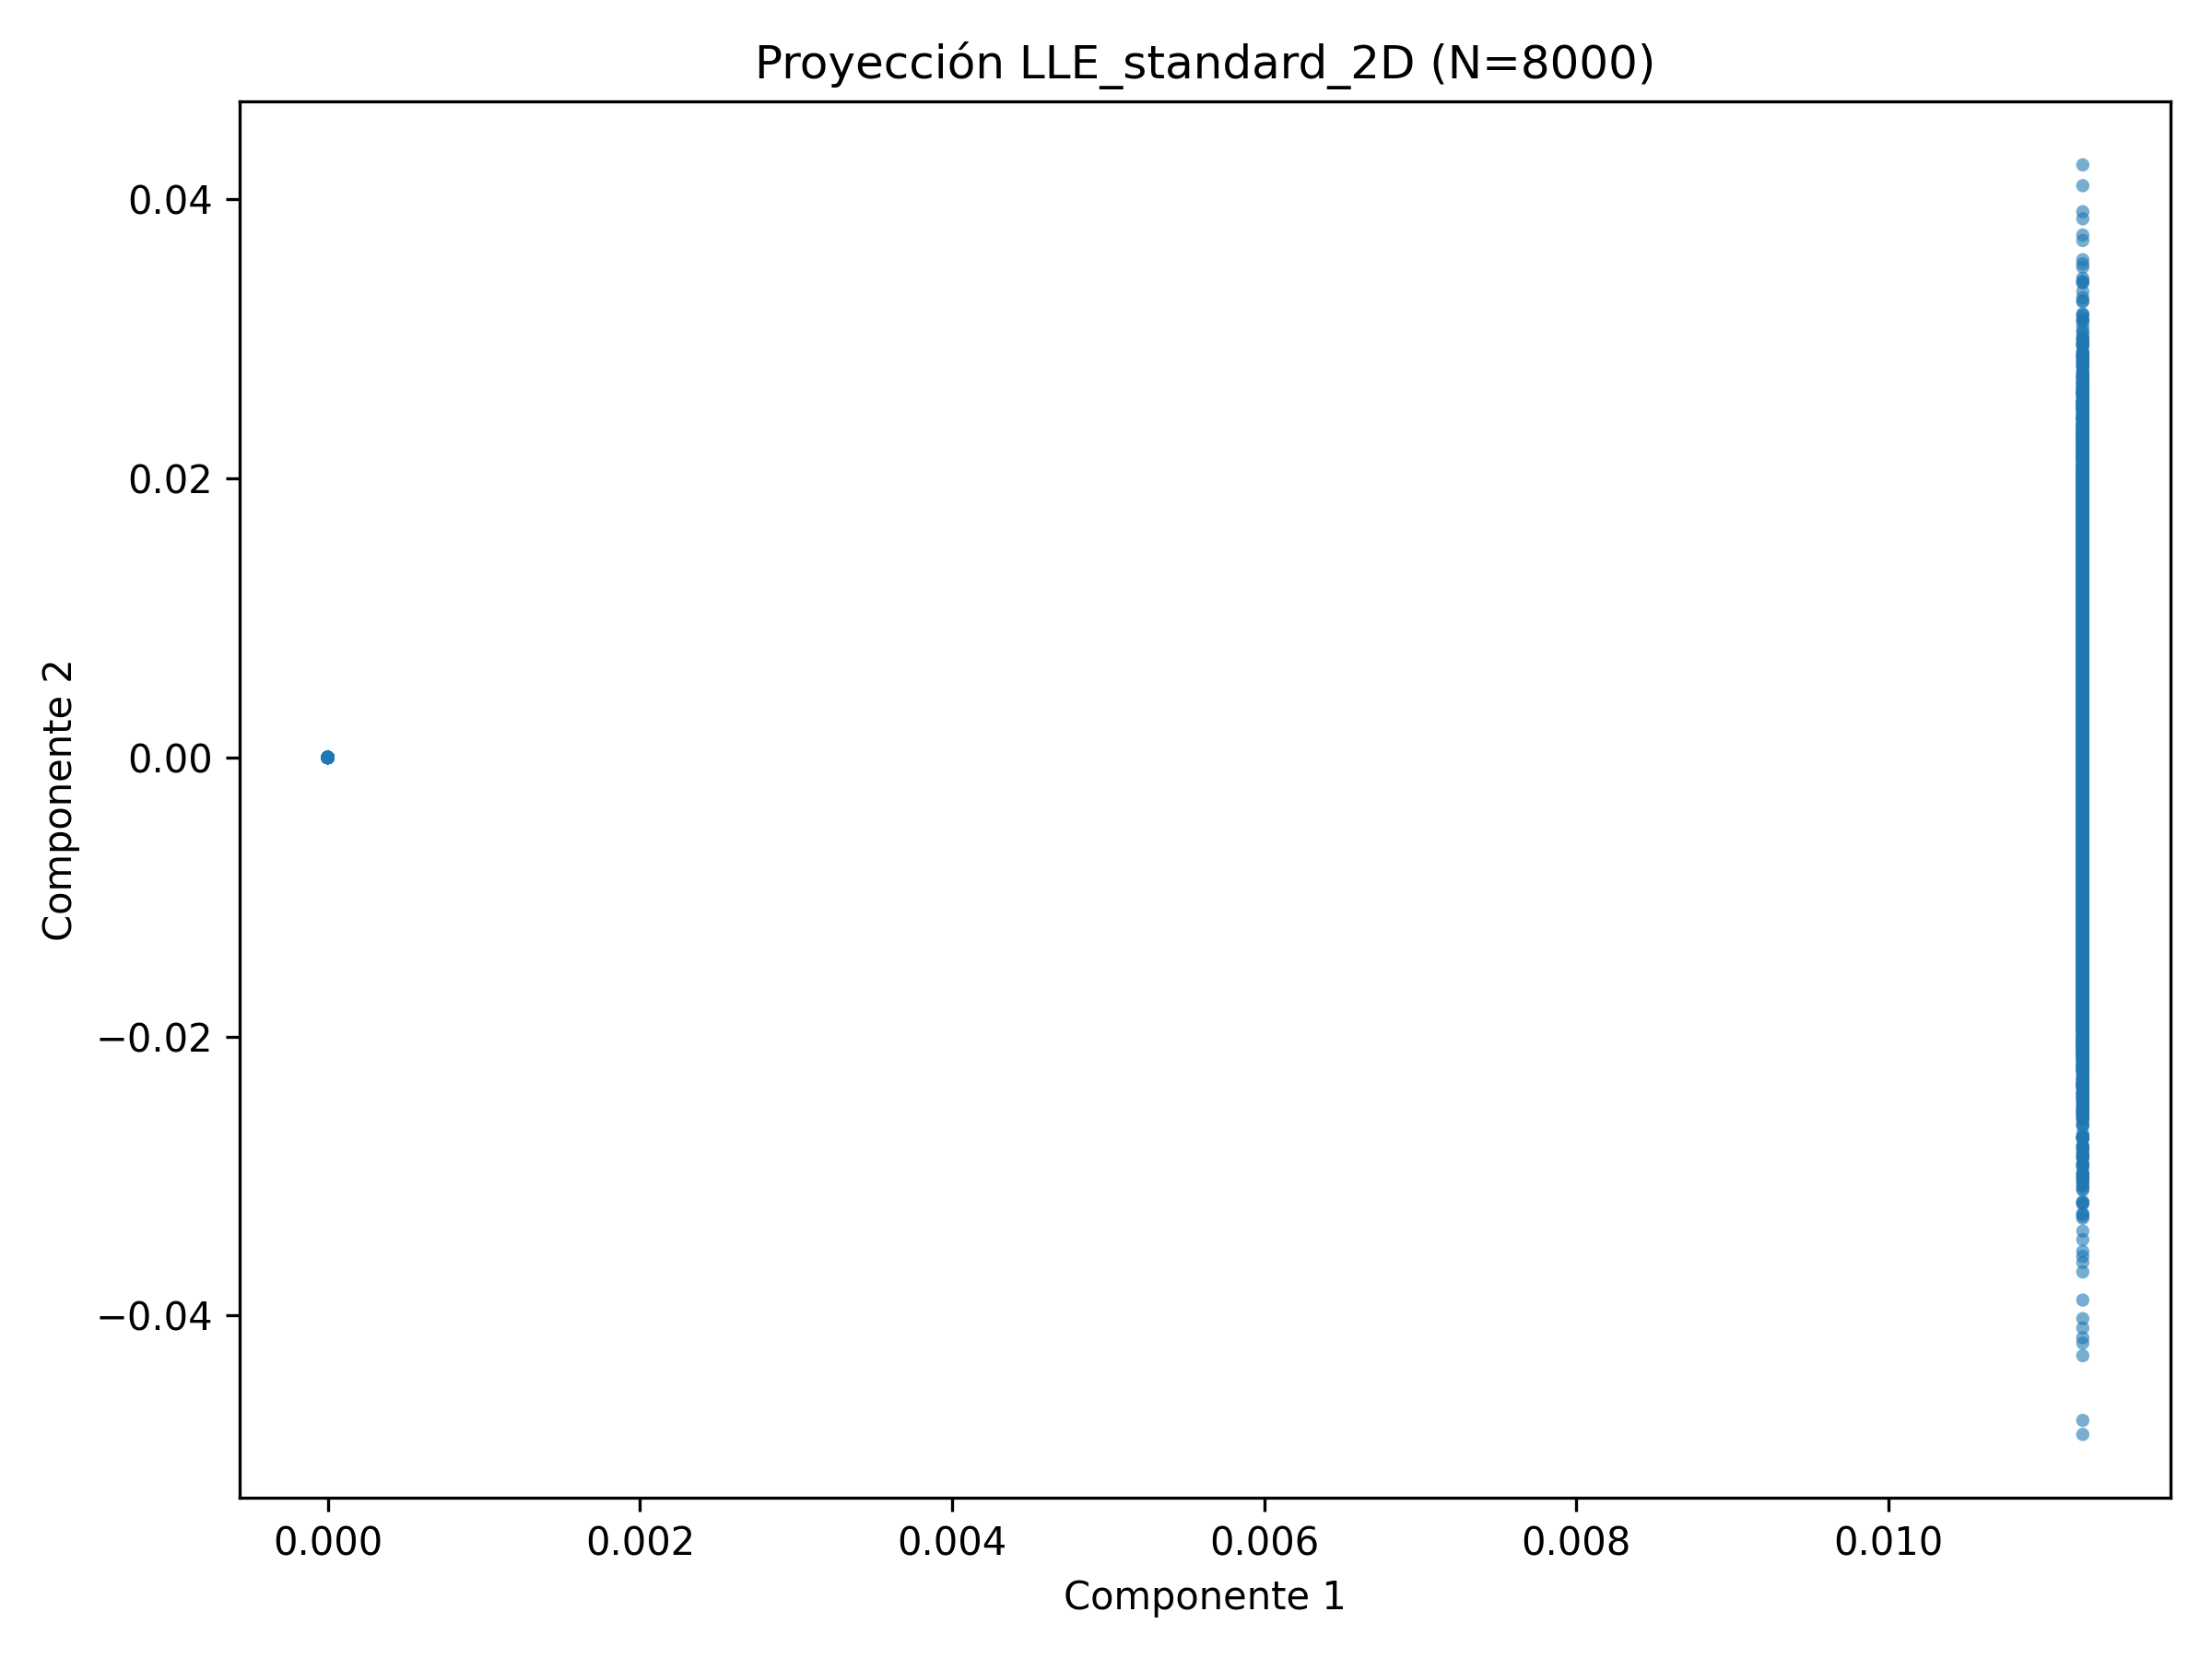
\includegraphics[width=\textwidth, height=0.75\textheight, keepaspectratio]{plot_LLE_standard_2D.png}
      \caption{\small Proyección LLE Standard 2D}
    \end{figure}
    
    \column{0.50\textwidth}
    \begin{figure}
      \centering
      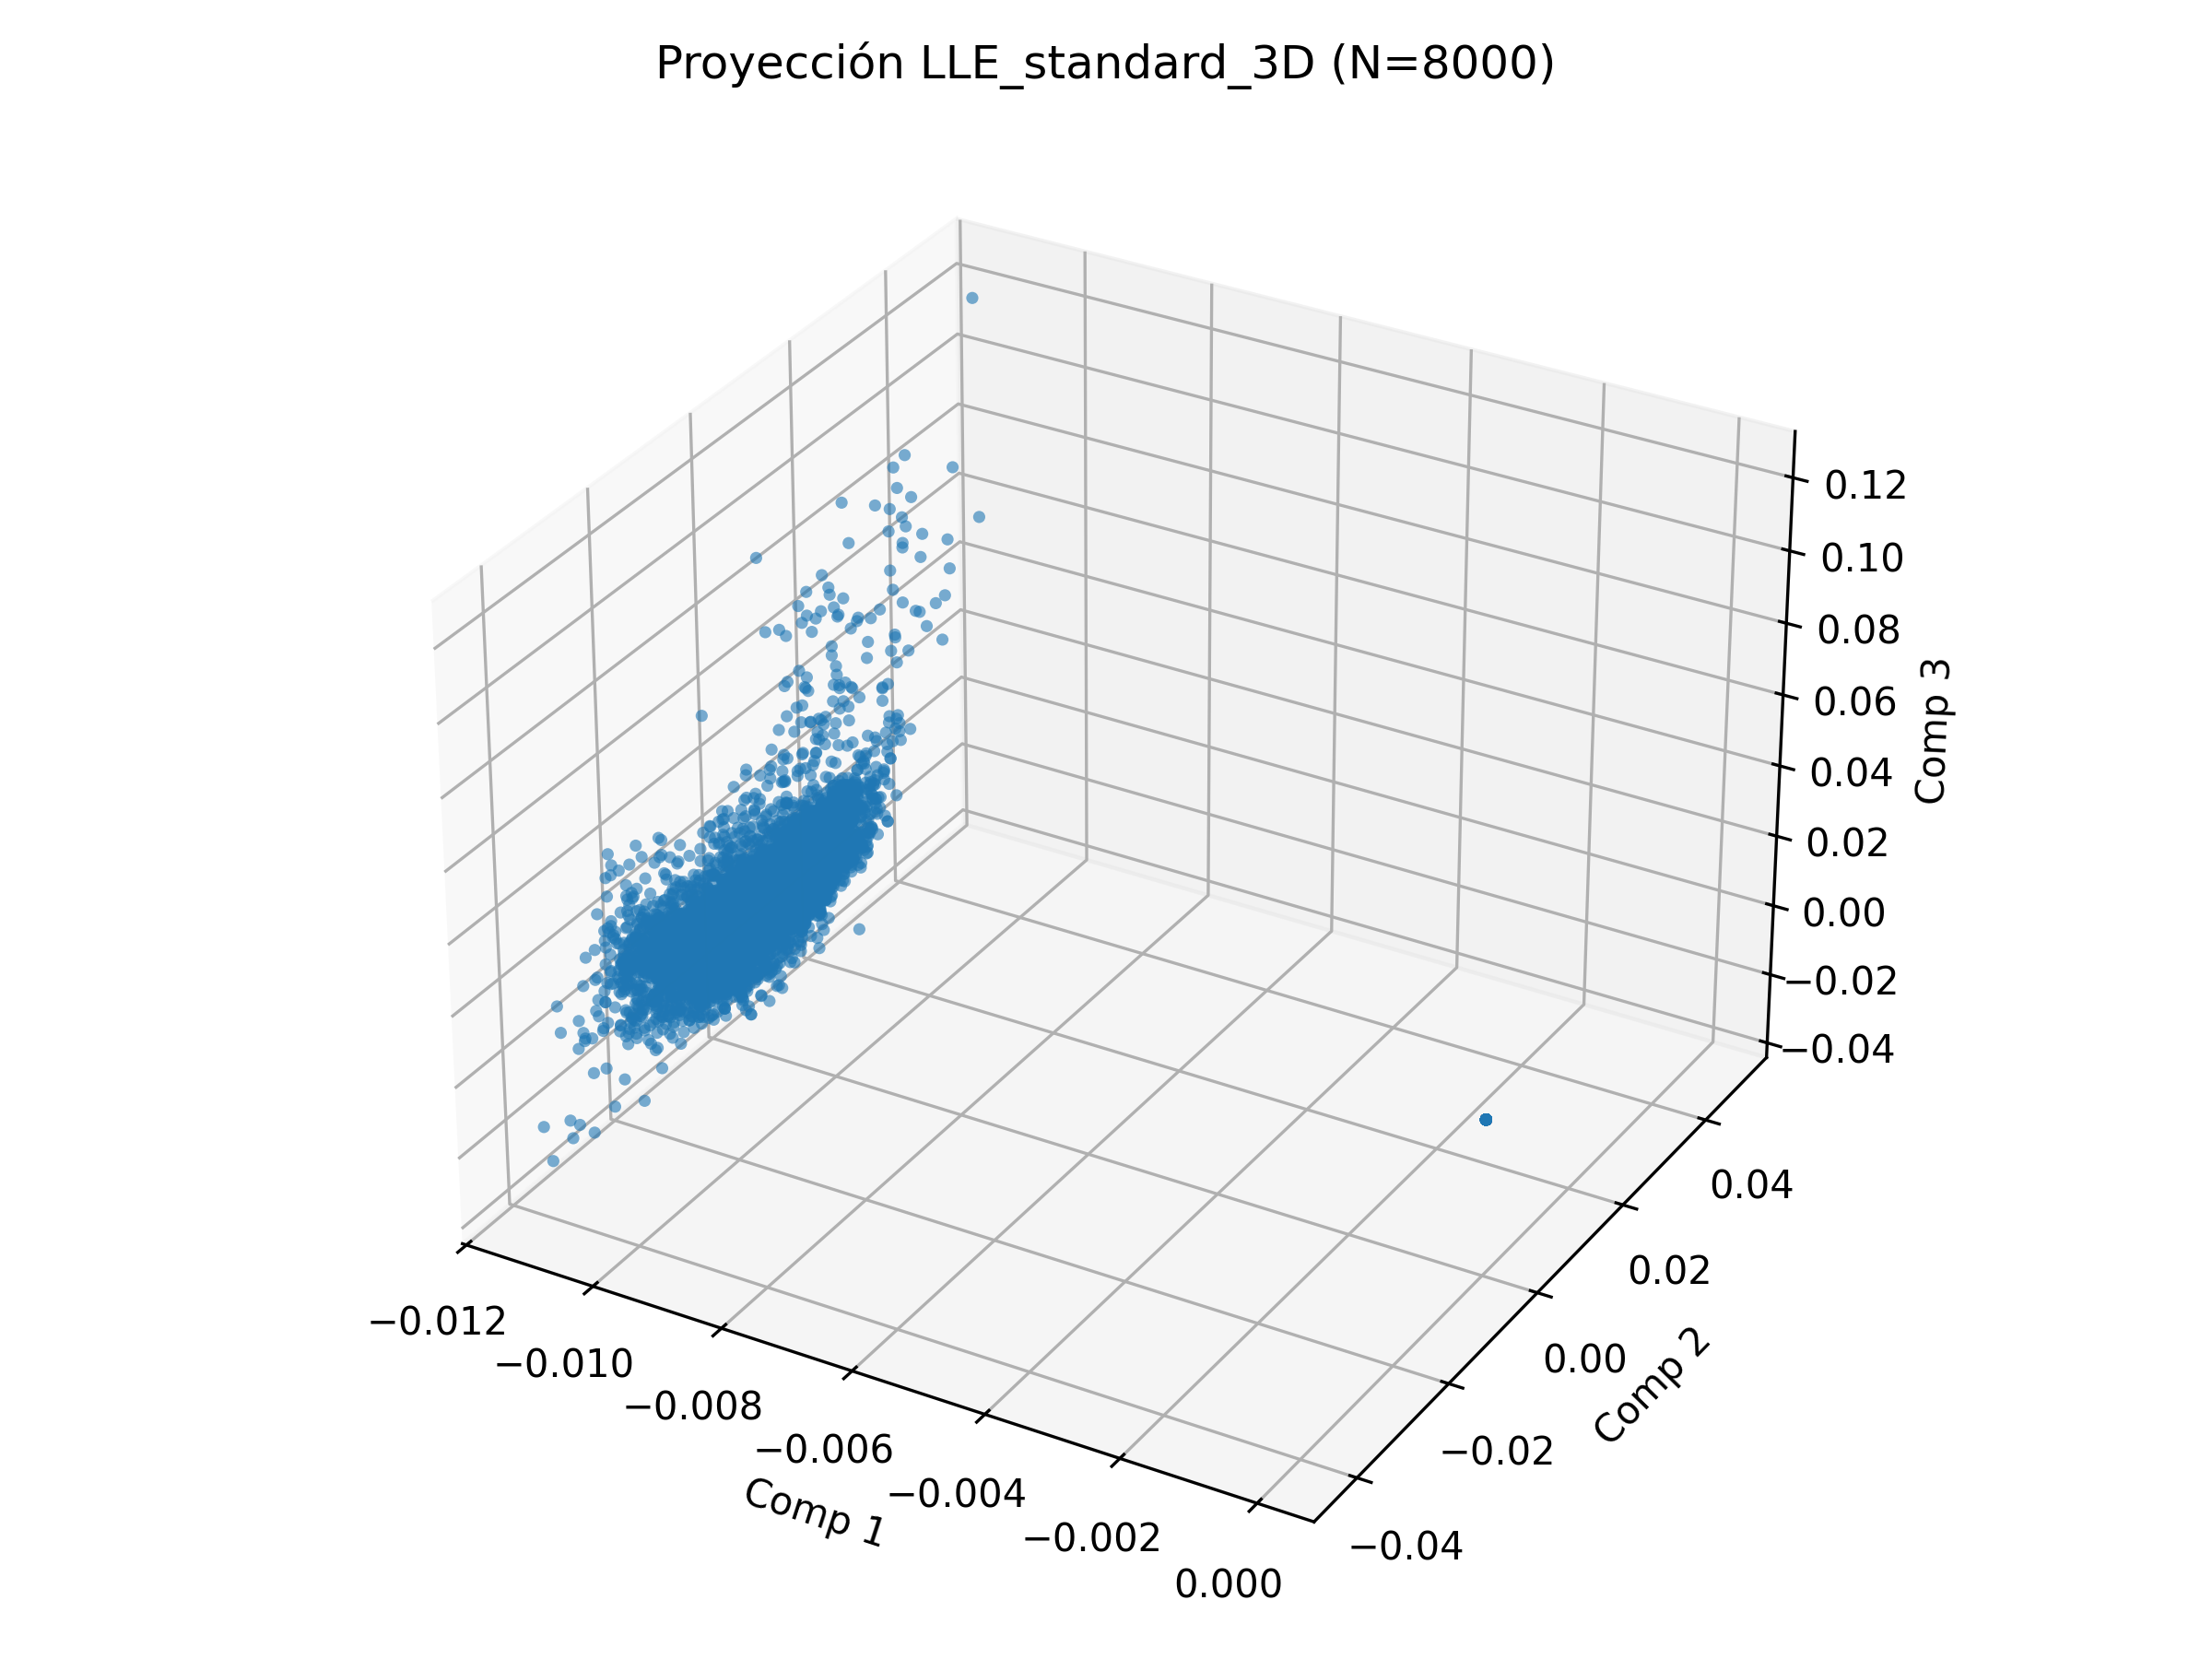
\includegraphics[width=\textwidth, height=0.75\textheight, keepaspectratio]{plot_LLE_standard_3D.png}
      \caption{\small Proyección LLE Standard 3D}
    \end{figure}
  \end{columns}
\end{frame}

% --- NCA ---
\begin{frame}{Experimento 3: Reducción de Dimensionalidad — NCA}
  \begin{columns}
    \column{0.50\textwidth}
    \begin{figure}
      \centering
      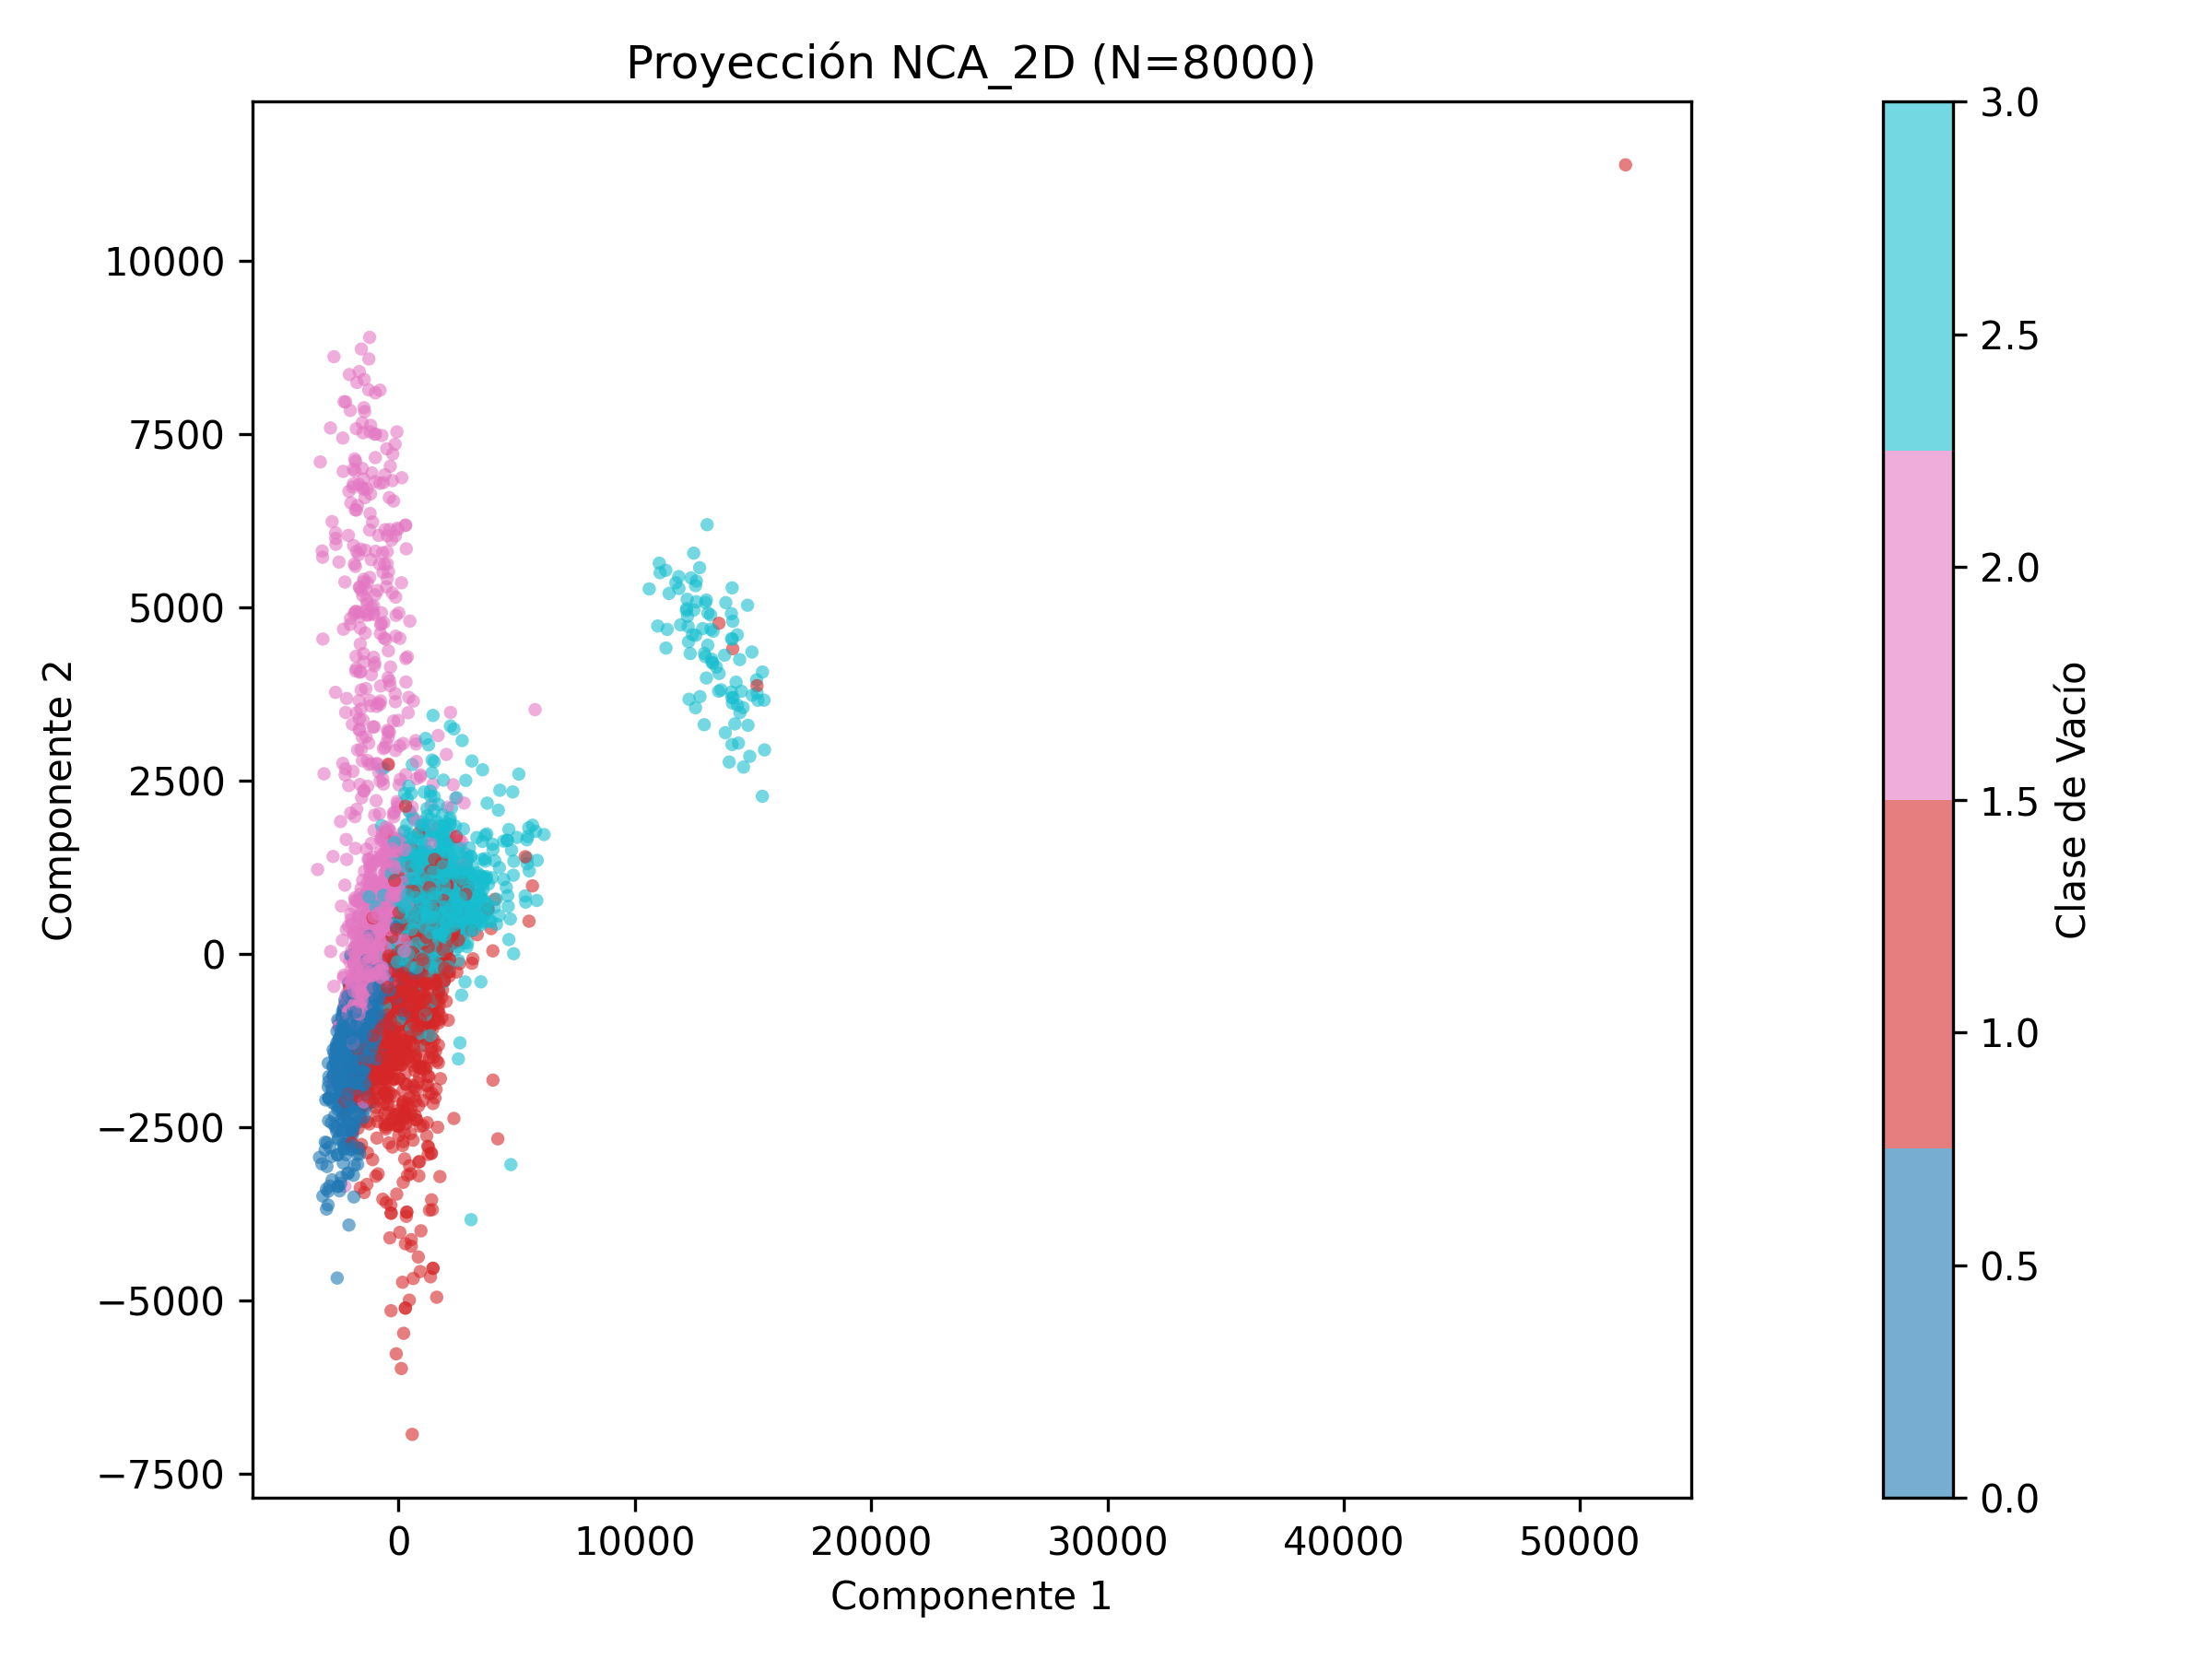
\includegraphics[width=\textwidth, height=0.75\textheight, keepaspectratio]{plot_NCA_2D.png}
      \caption{\small Proyección NCA 2D}
    \end{figure}
    
    \column{0.50\textwidth}
    \begin{figure}
      \centering
      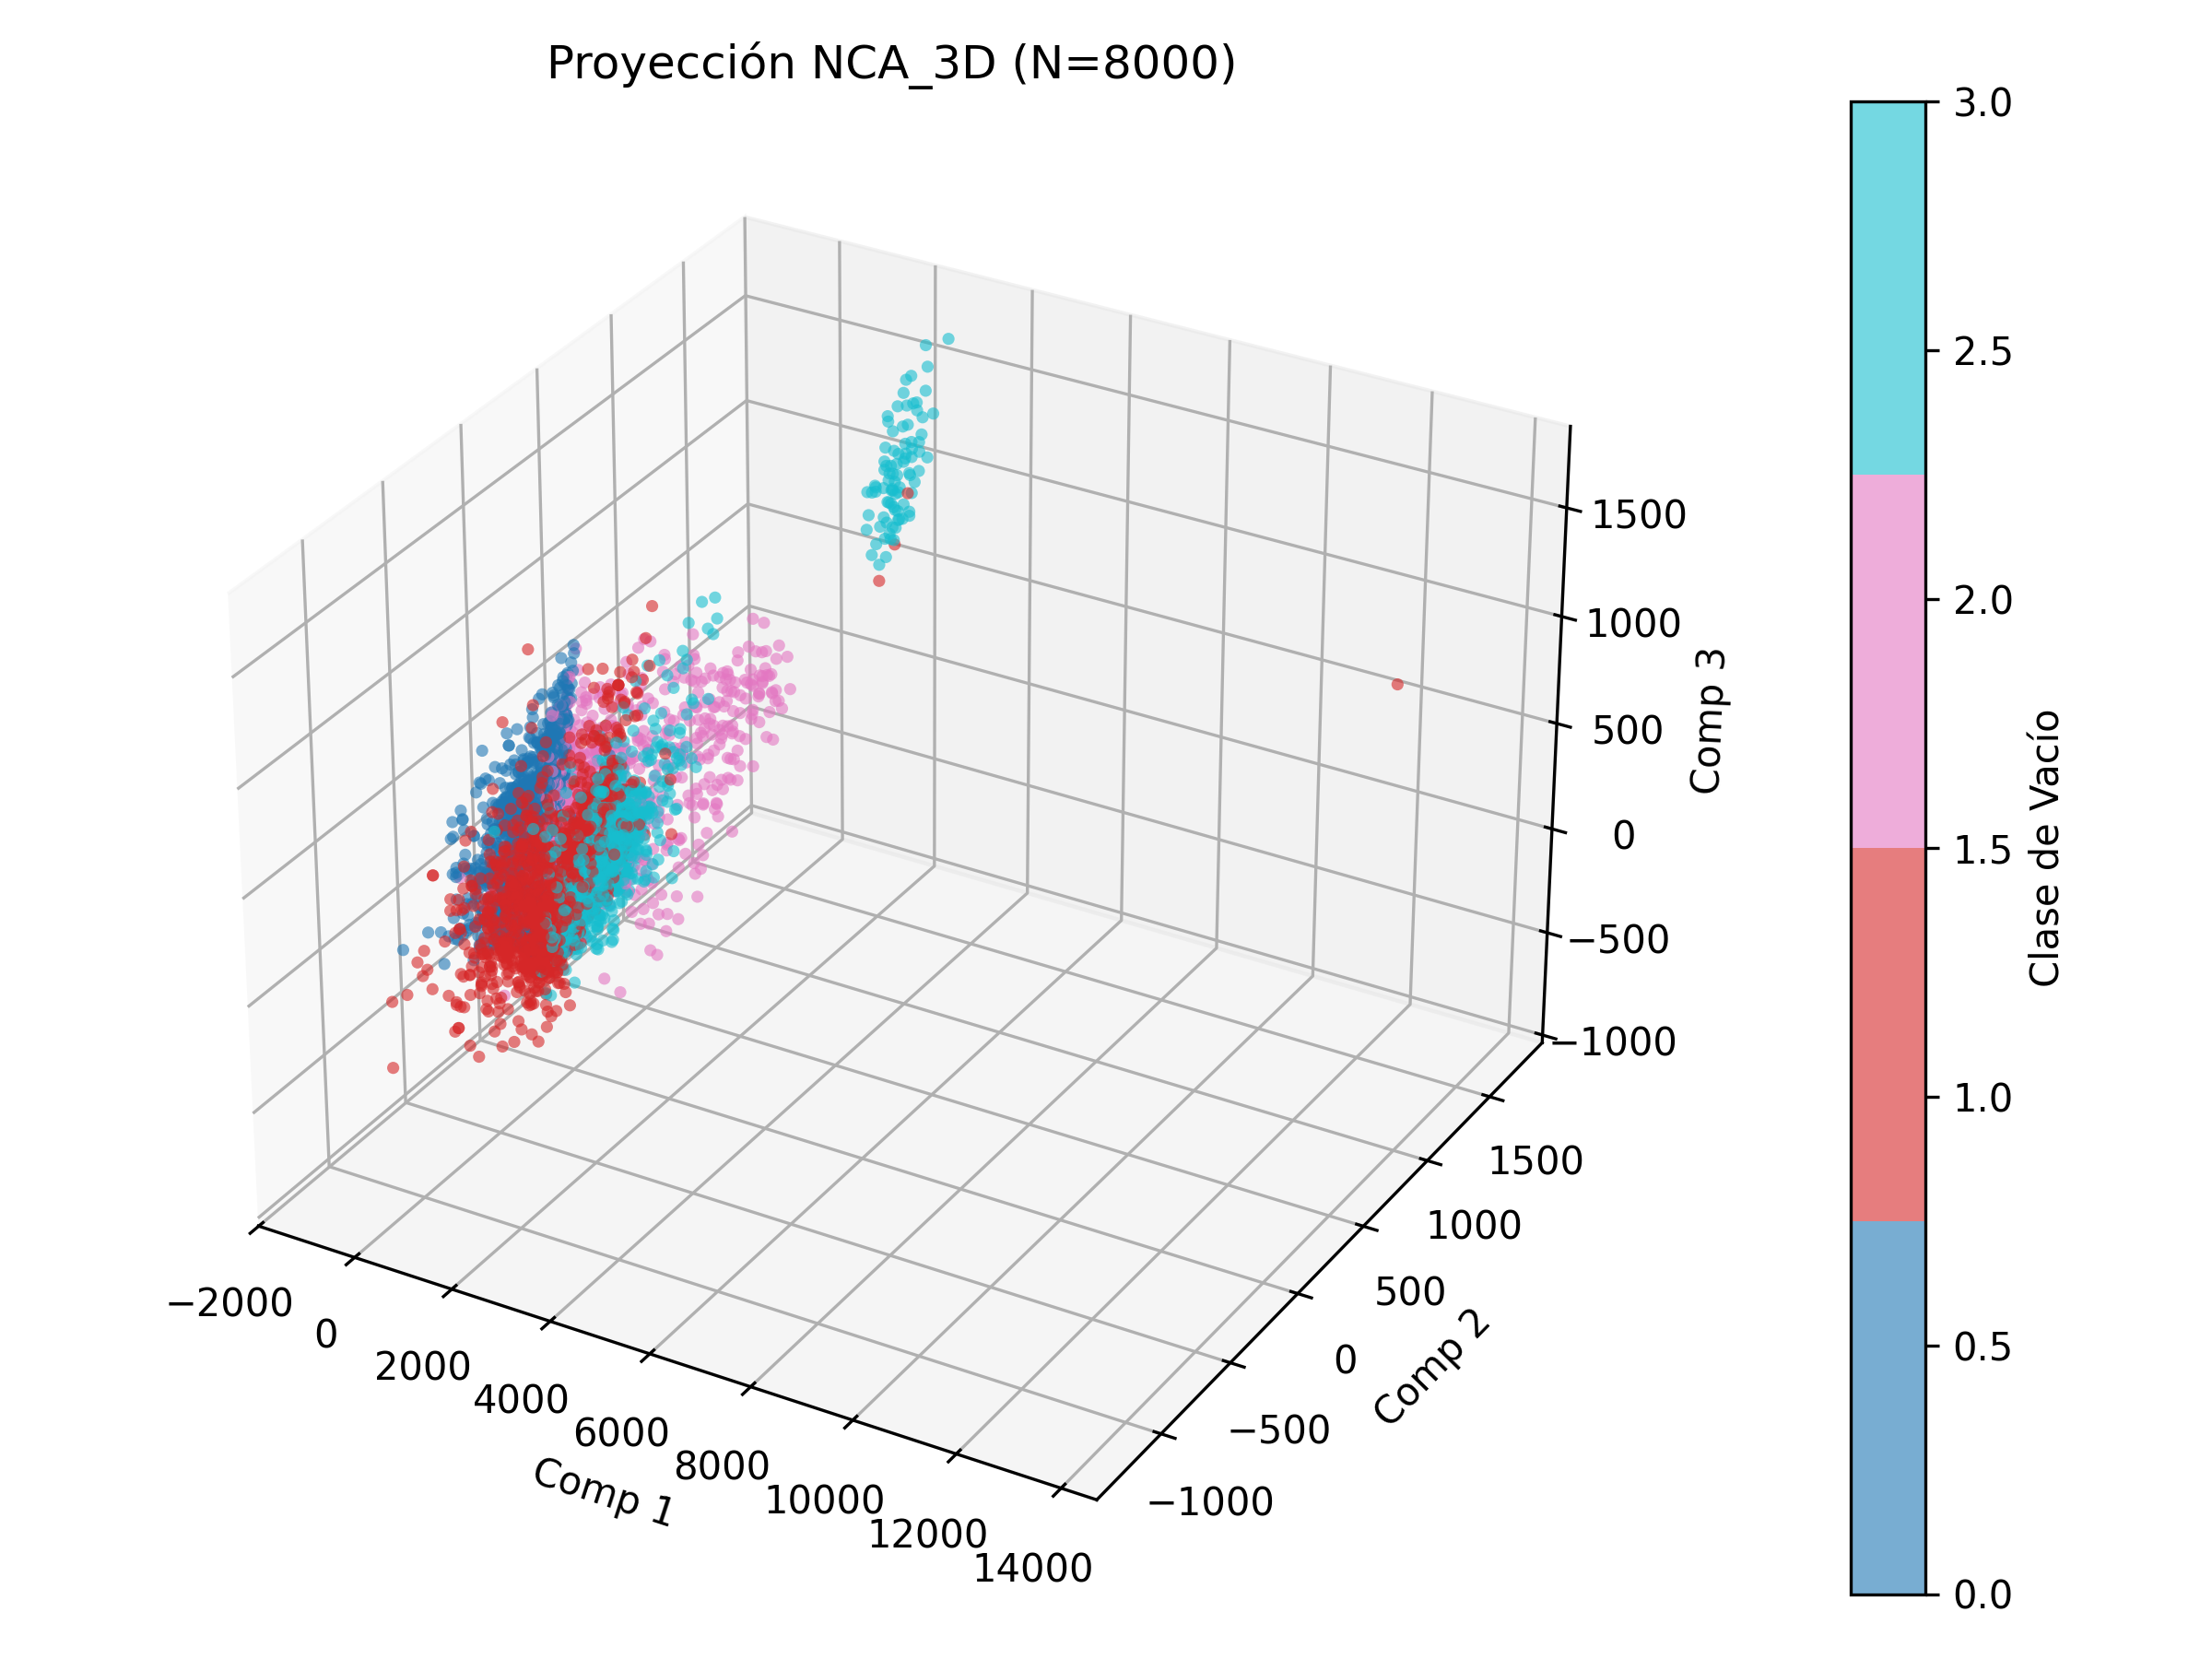
\includegraphics[width=\textwidth, height=0.75\textheight, keepaspectratio]{plot_NCA_3D.png}
      \caption{\small Proyección NCA 3D}
    \end{figure}
  \end{columns}
\end{frame}

% --- PCA ---
\begin{frame}{Experimento 3: Reducción de Dimensionalidad — PCA}
  \begin{columns}
    \column{0.50\textwidth}
    \begin{figure}
      \centering
      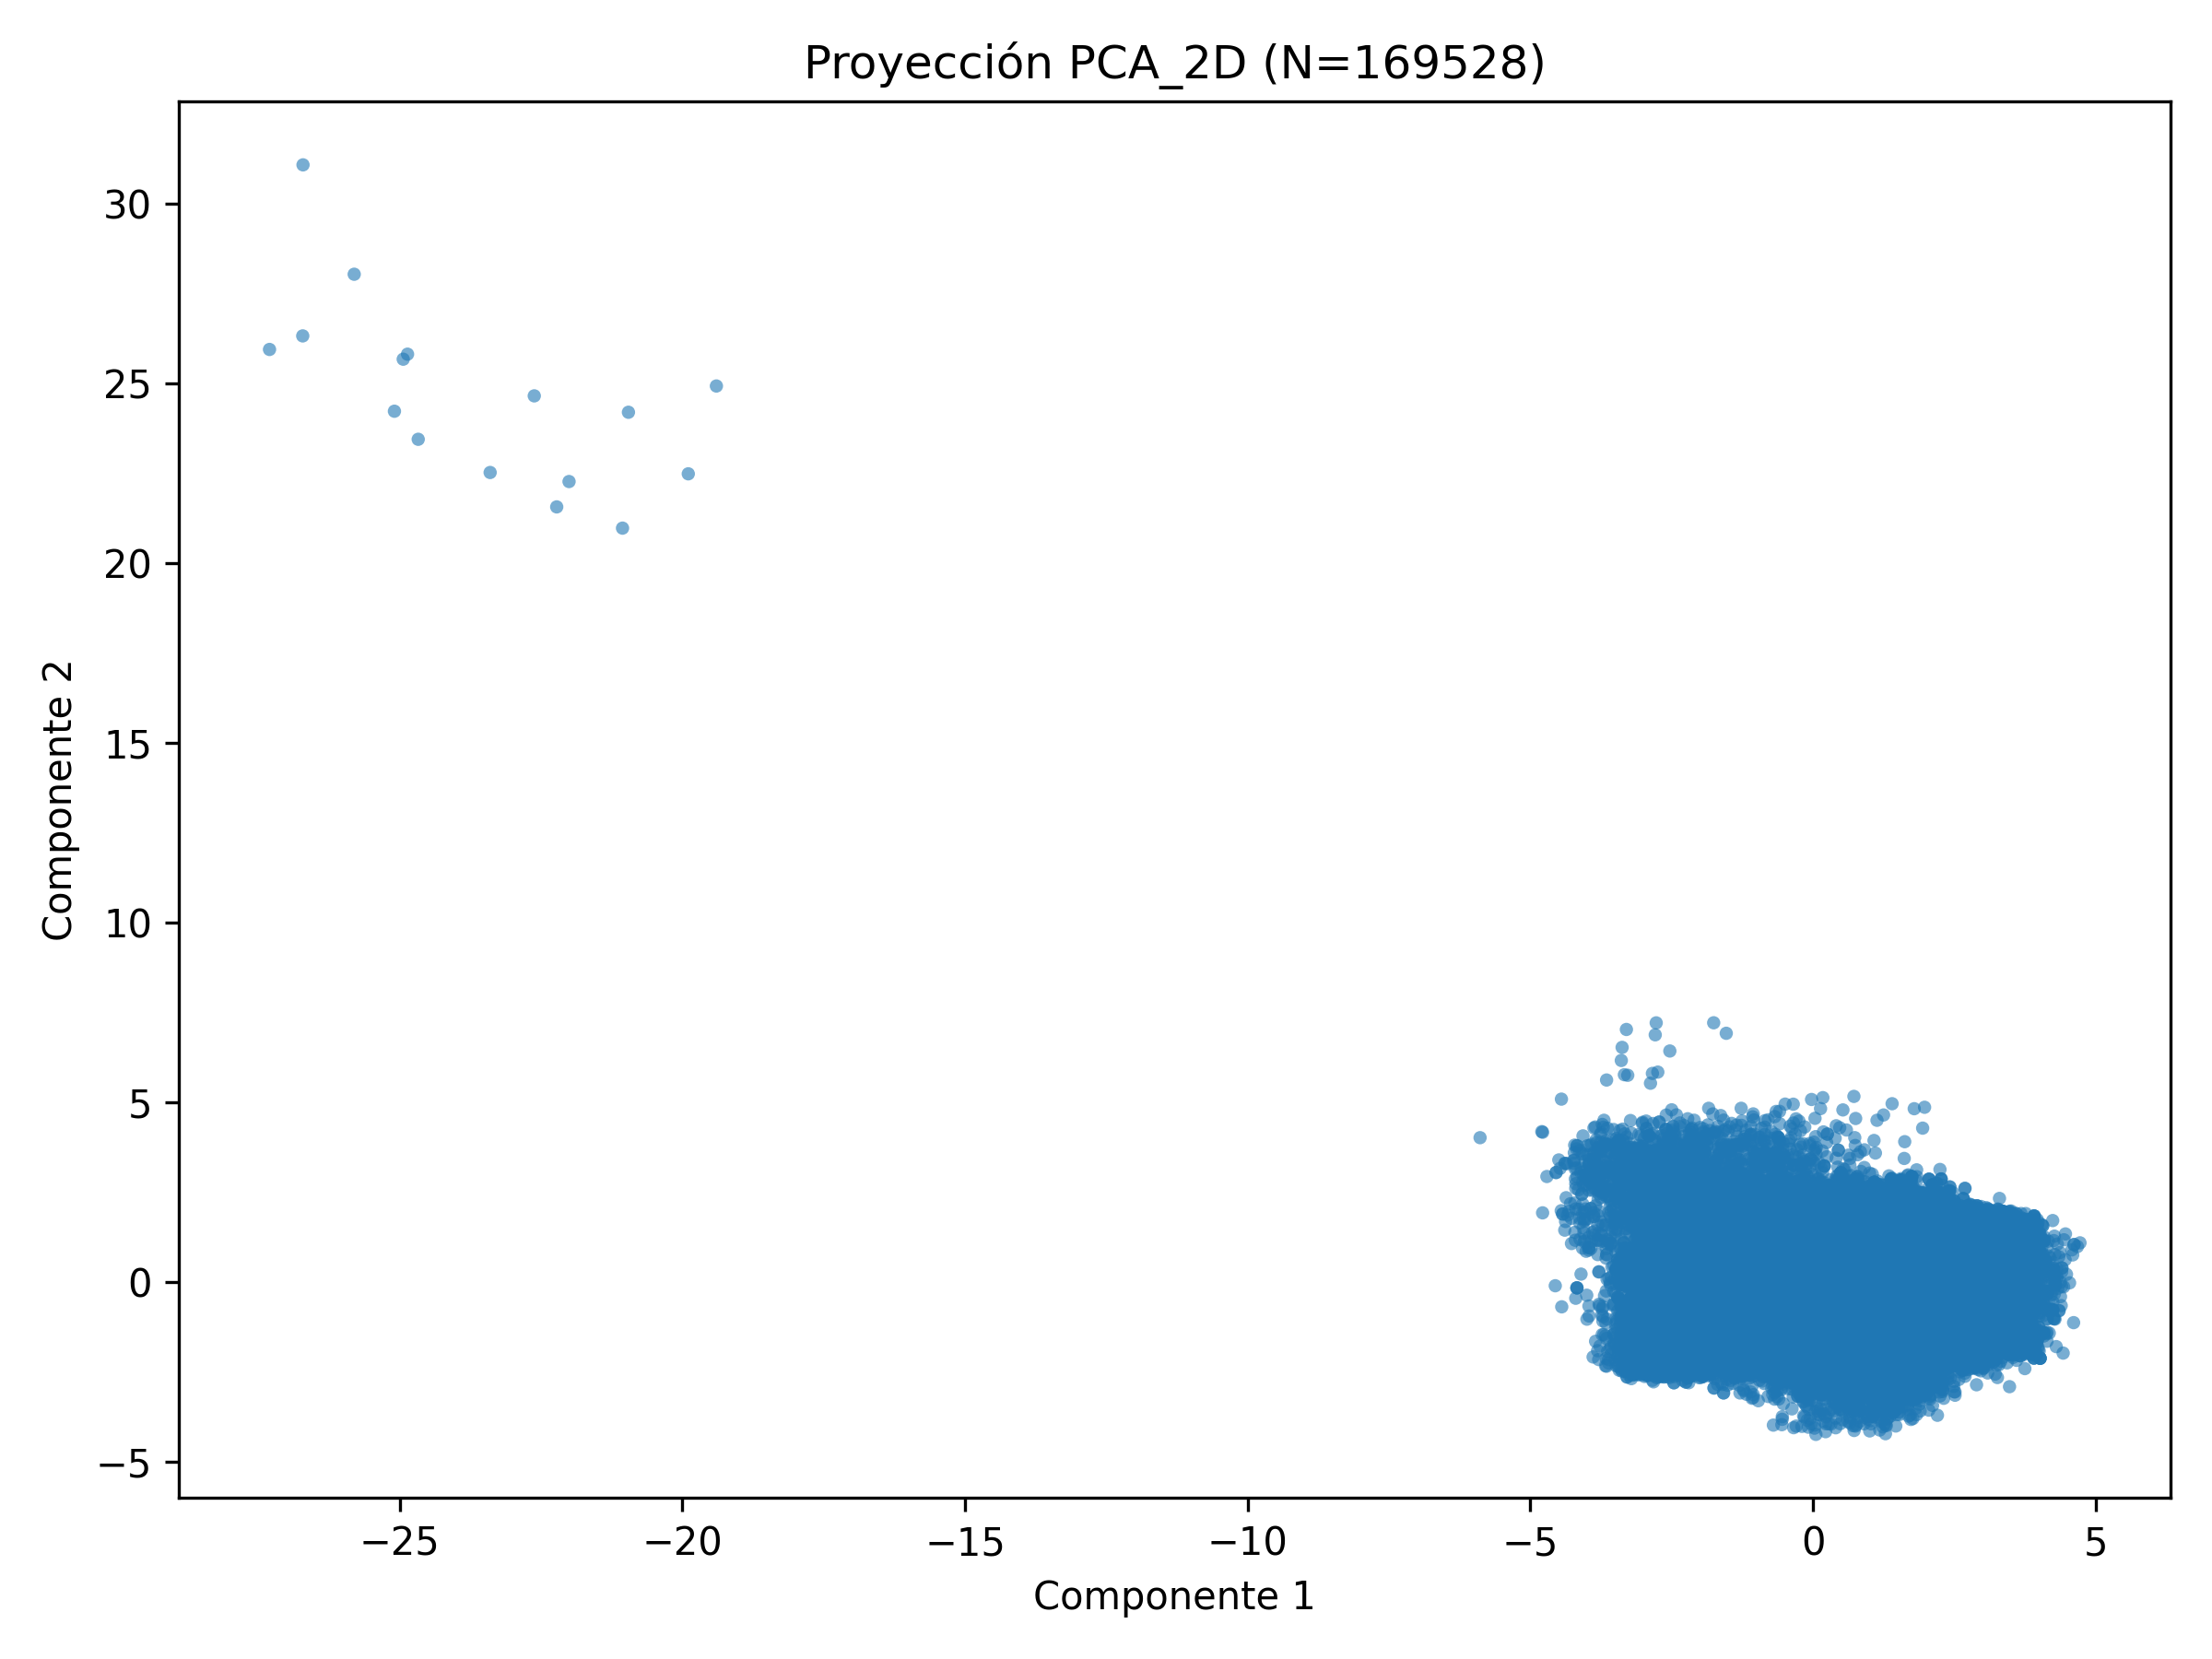
\includegraphics[width=\textwidth, height=0.75\textheight, keepaspectratio]{plot_PCA_2D.png}
      \caption{\small Proyección PCA 2D}
    \end{figure}
    
    \column{0.50\textwidth}
    \begin{figure}
      \centering
      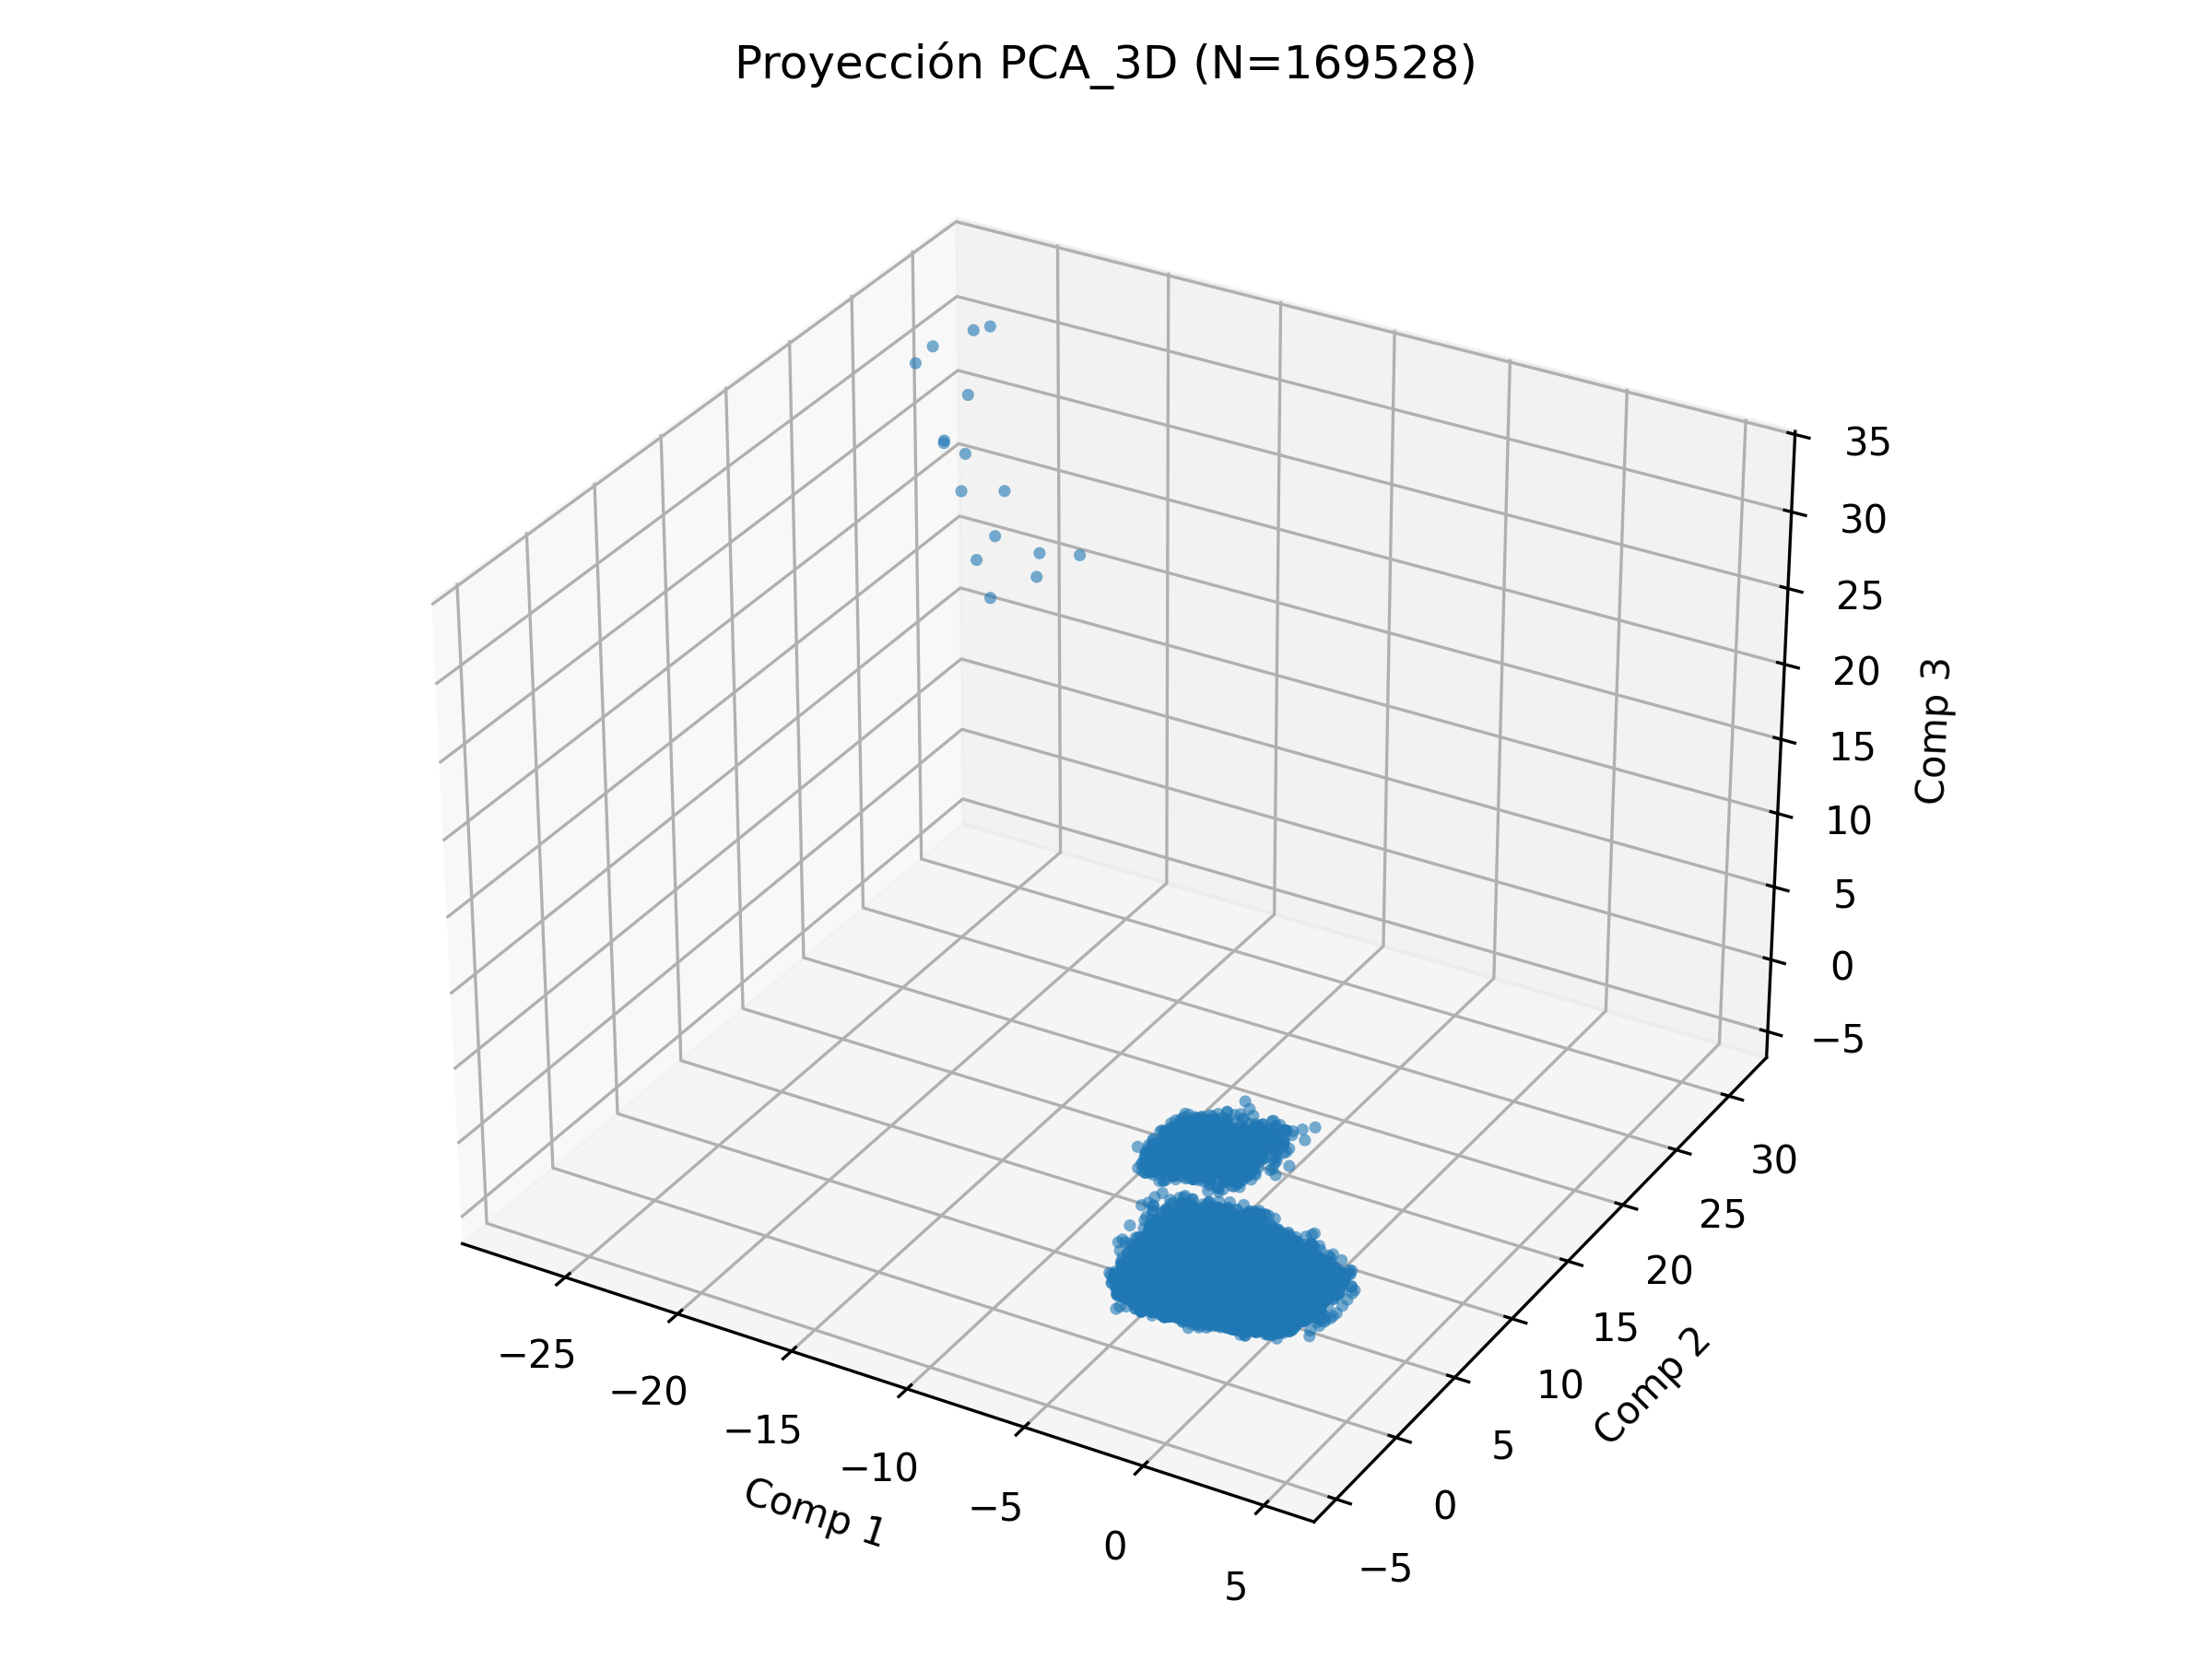
\includegraphics[width=\textwidth, height=0.75\textheight, keepaspectratio]{plot_PCA_3D.png}
      \caption{\small Proyección PCA 3D}
    \end{figure}
  \end{columns}
\end{frame}

% --- SparsePCA ---
\begin{frame}{Experimento 3: Reducción de Dimensionalidad — Sparse PCA}
  \begin{columns}
    \column{0.50\textwidth}
    \begin{figure}
      \centering
      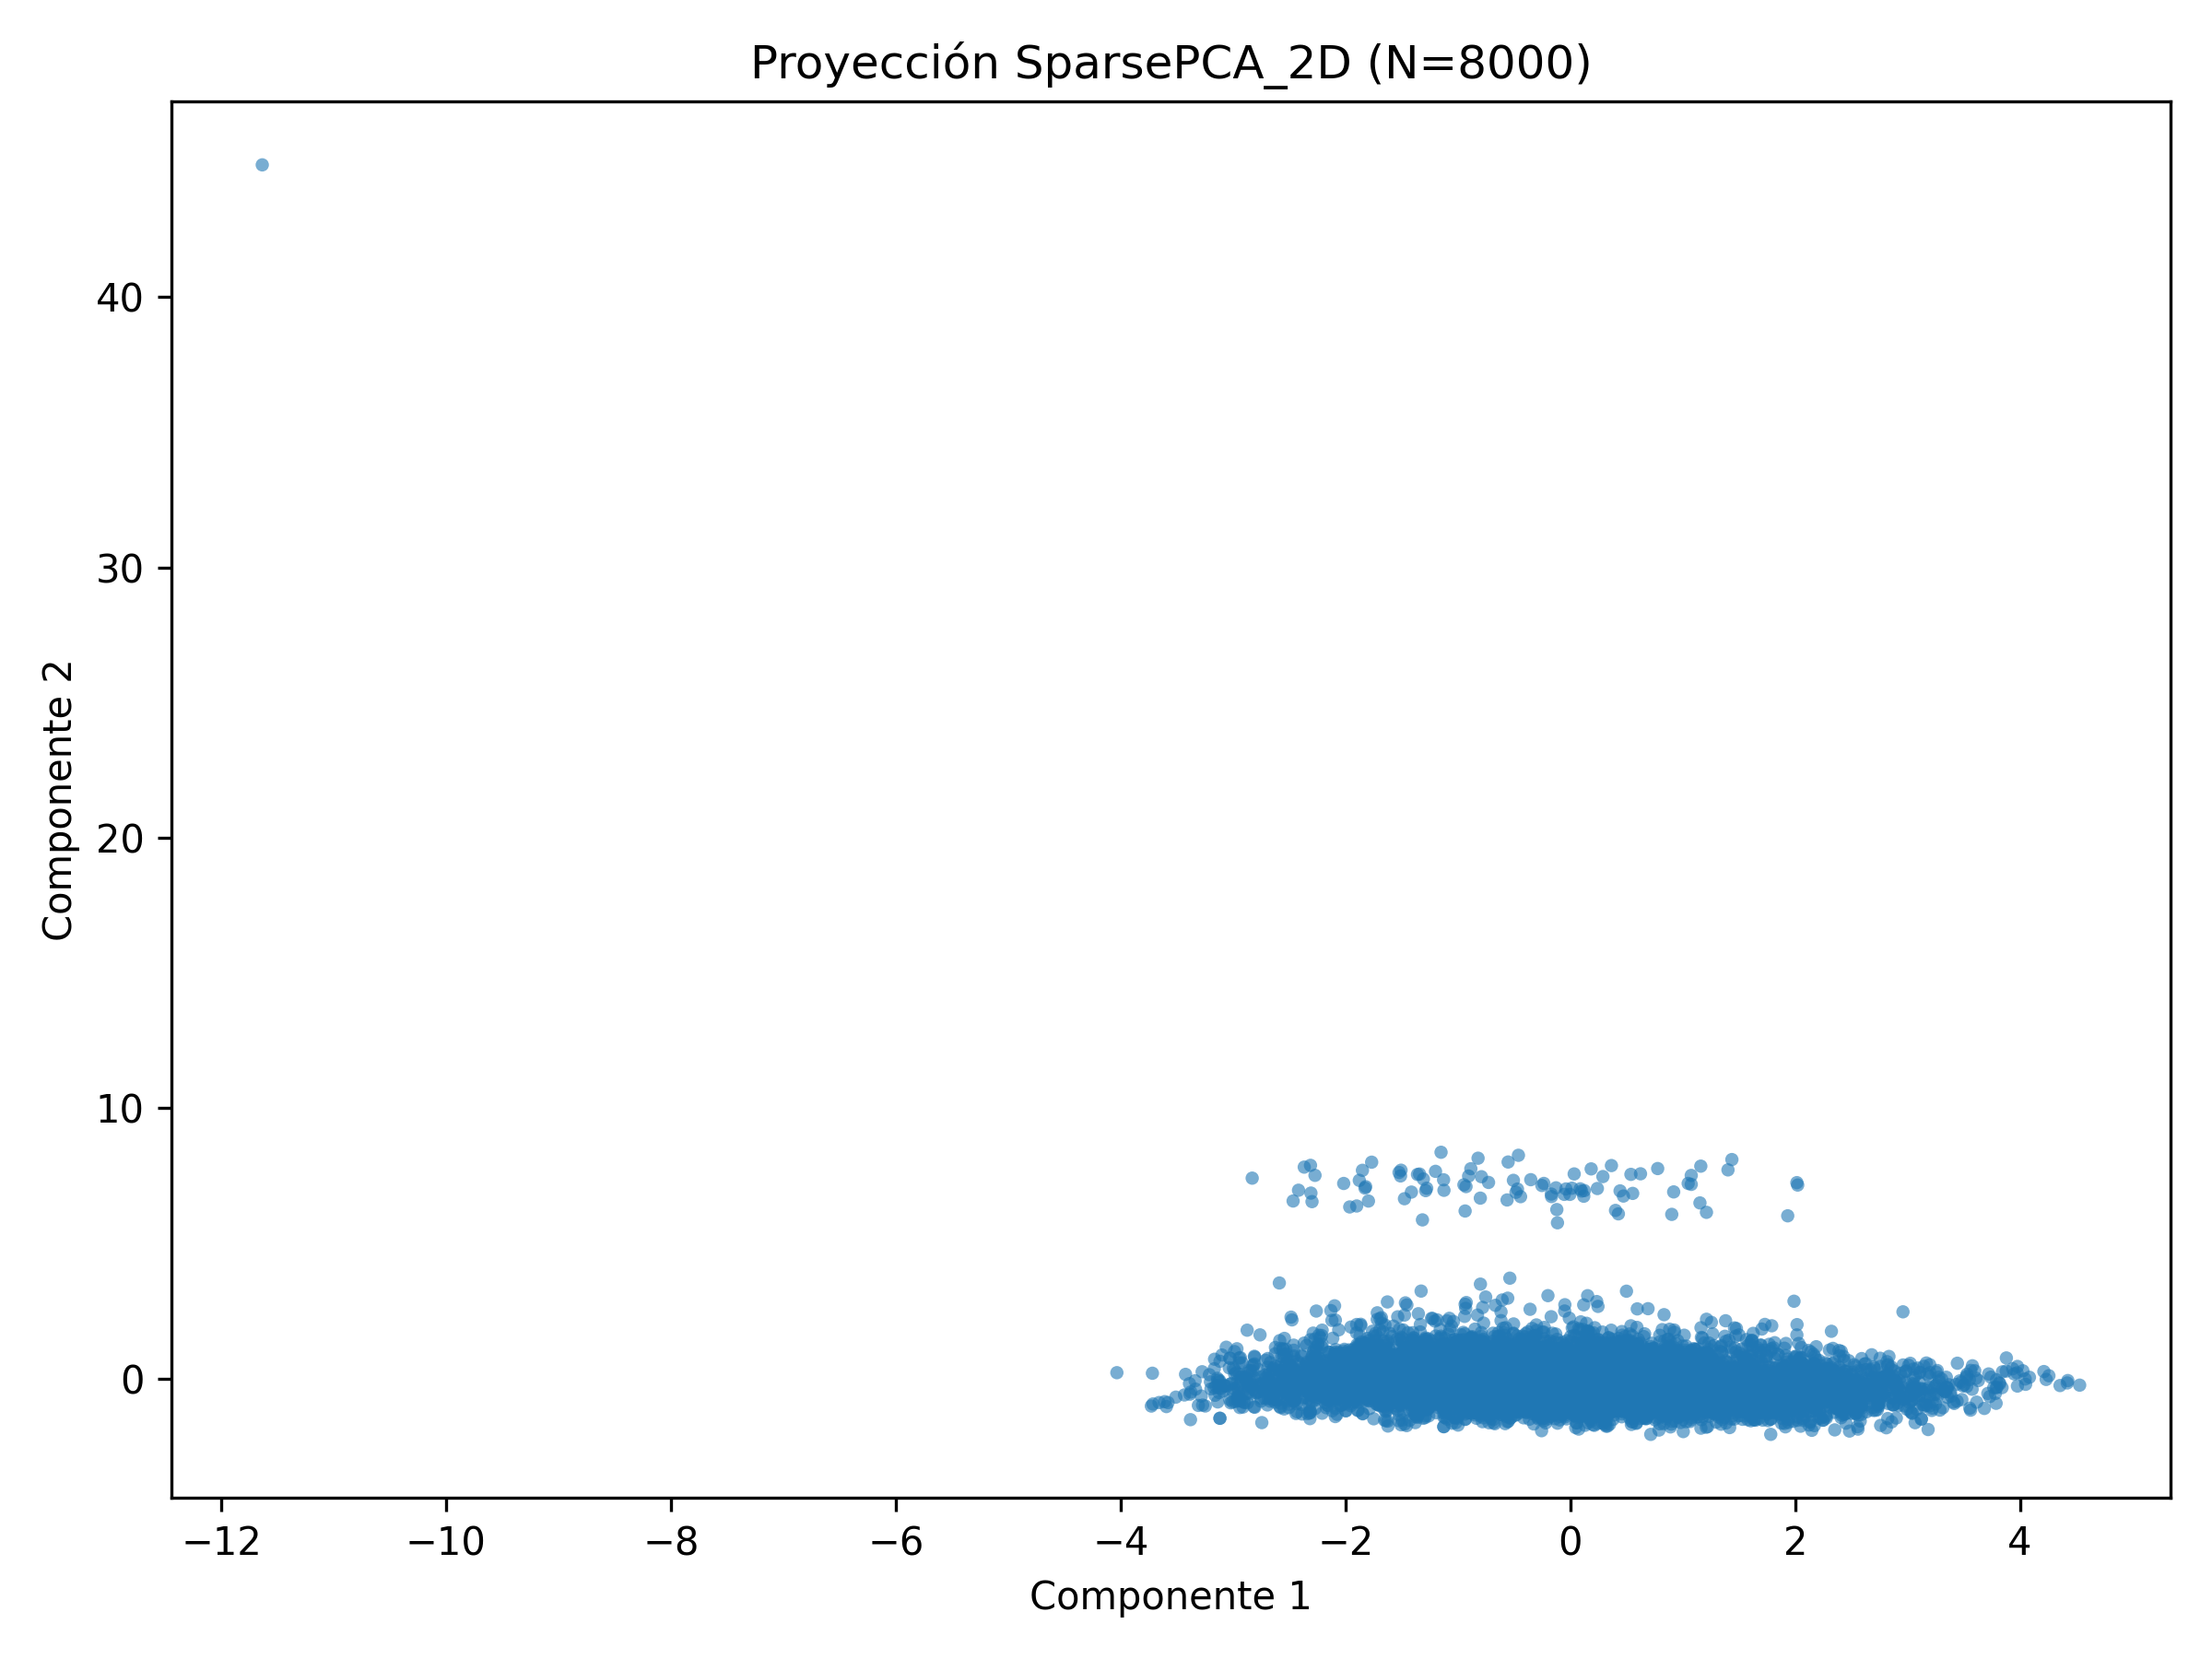
\includegraphics[width=\textwidth, height=0.75\textheight, keepaspectratio]{plot_SparsePCA_2D.png}
      \caption{\small Proyección Sparse PCA 2D}
    \end{figure}
    
    \column{0.50\textwidth}
    \begin{figure}
      \centering
      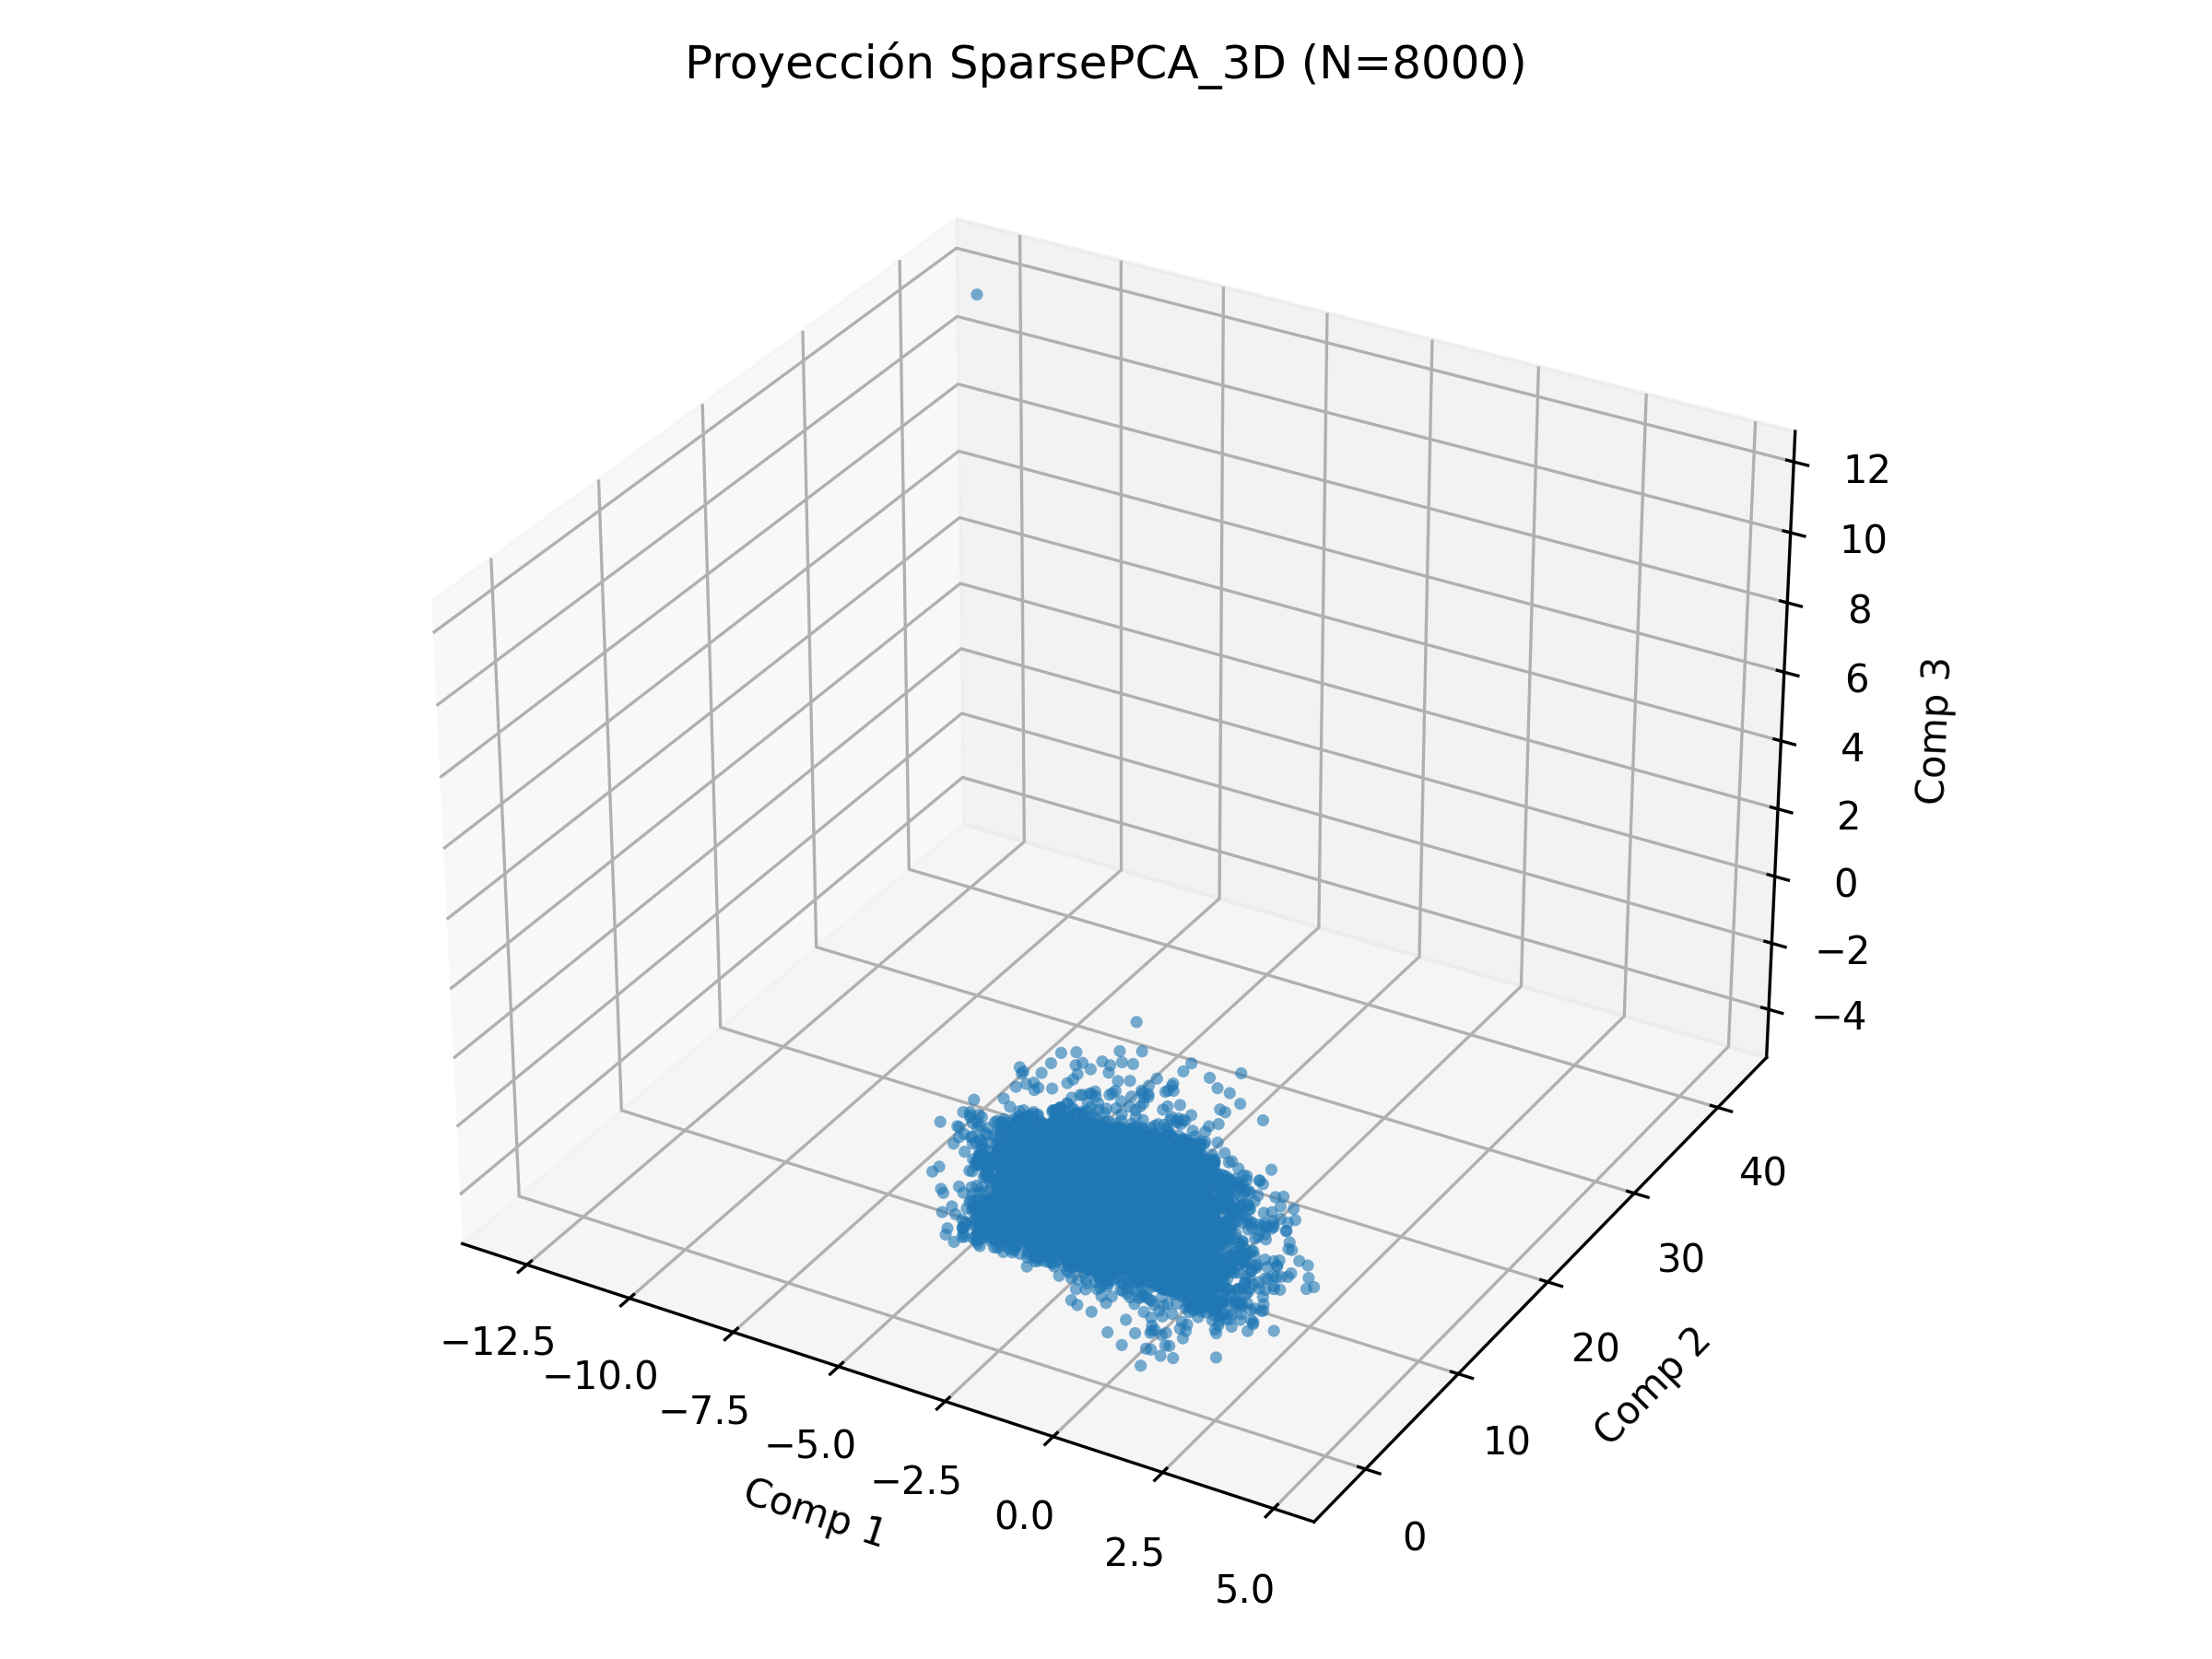
\includegraphics[width=\textwidth, height=0.75\textheight, keepaspectratio]{plot_SparsePCA_3D.png}
      \caption{\small Proyección Sparse PCA 3D}
    \end{figure}
  \end{columns}
\end{frame}

% --- TruncatedSVD ---
\begin{frame}{Experimento 3: Reducción de Dimensionalidad — Truncated SVD}
  \begin{columns}
    \column{0.50\textwidth}
    \begin{figure}
      \centering
      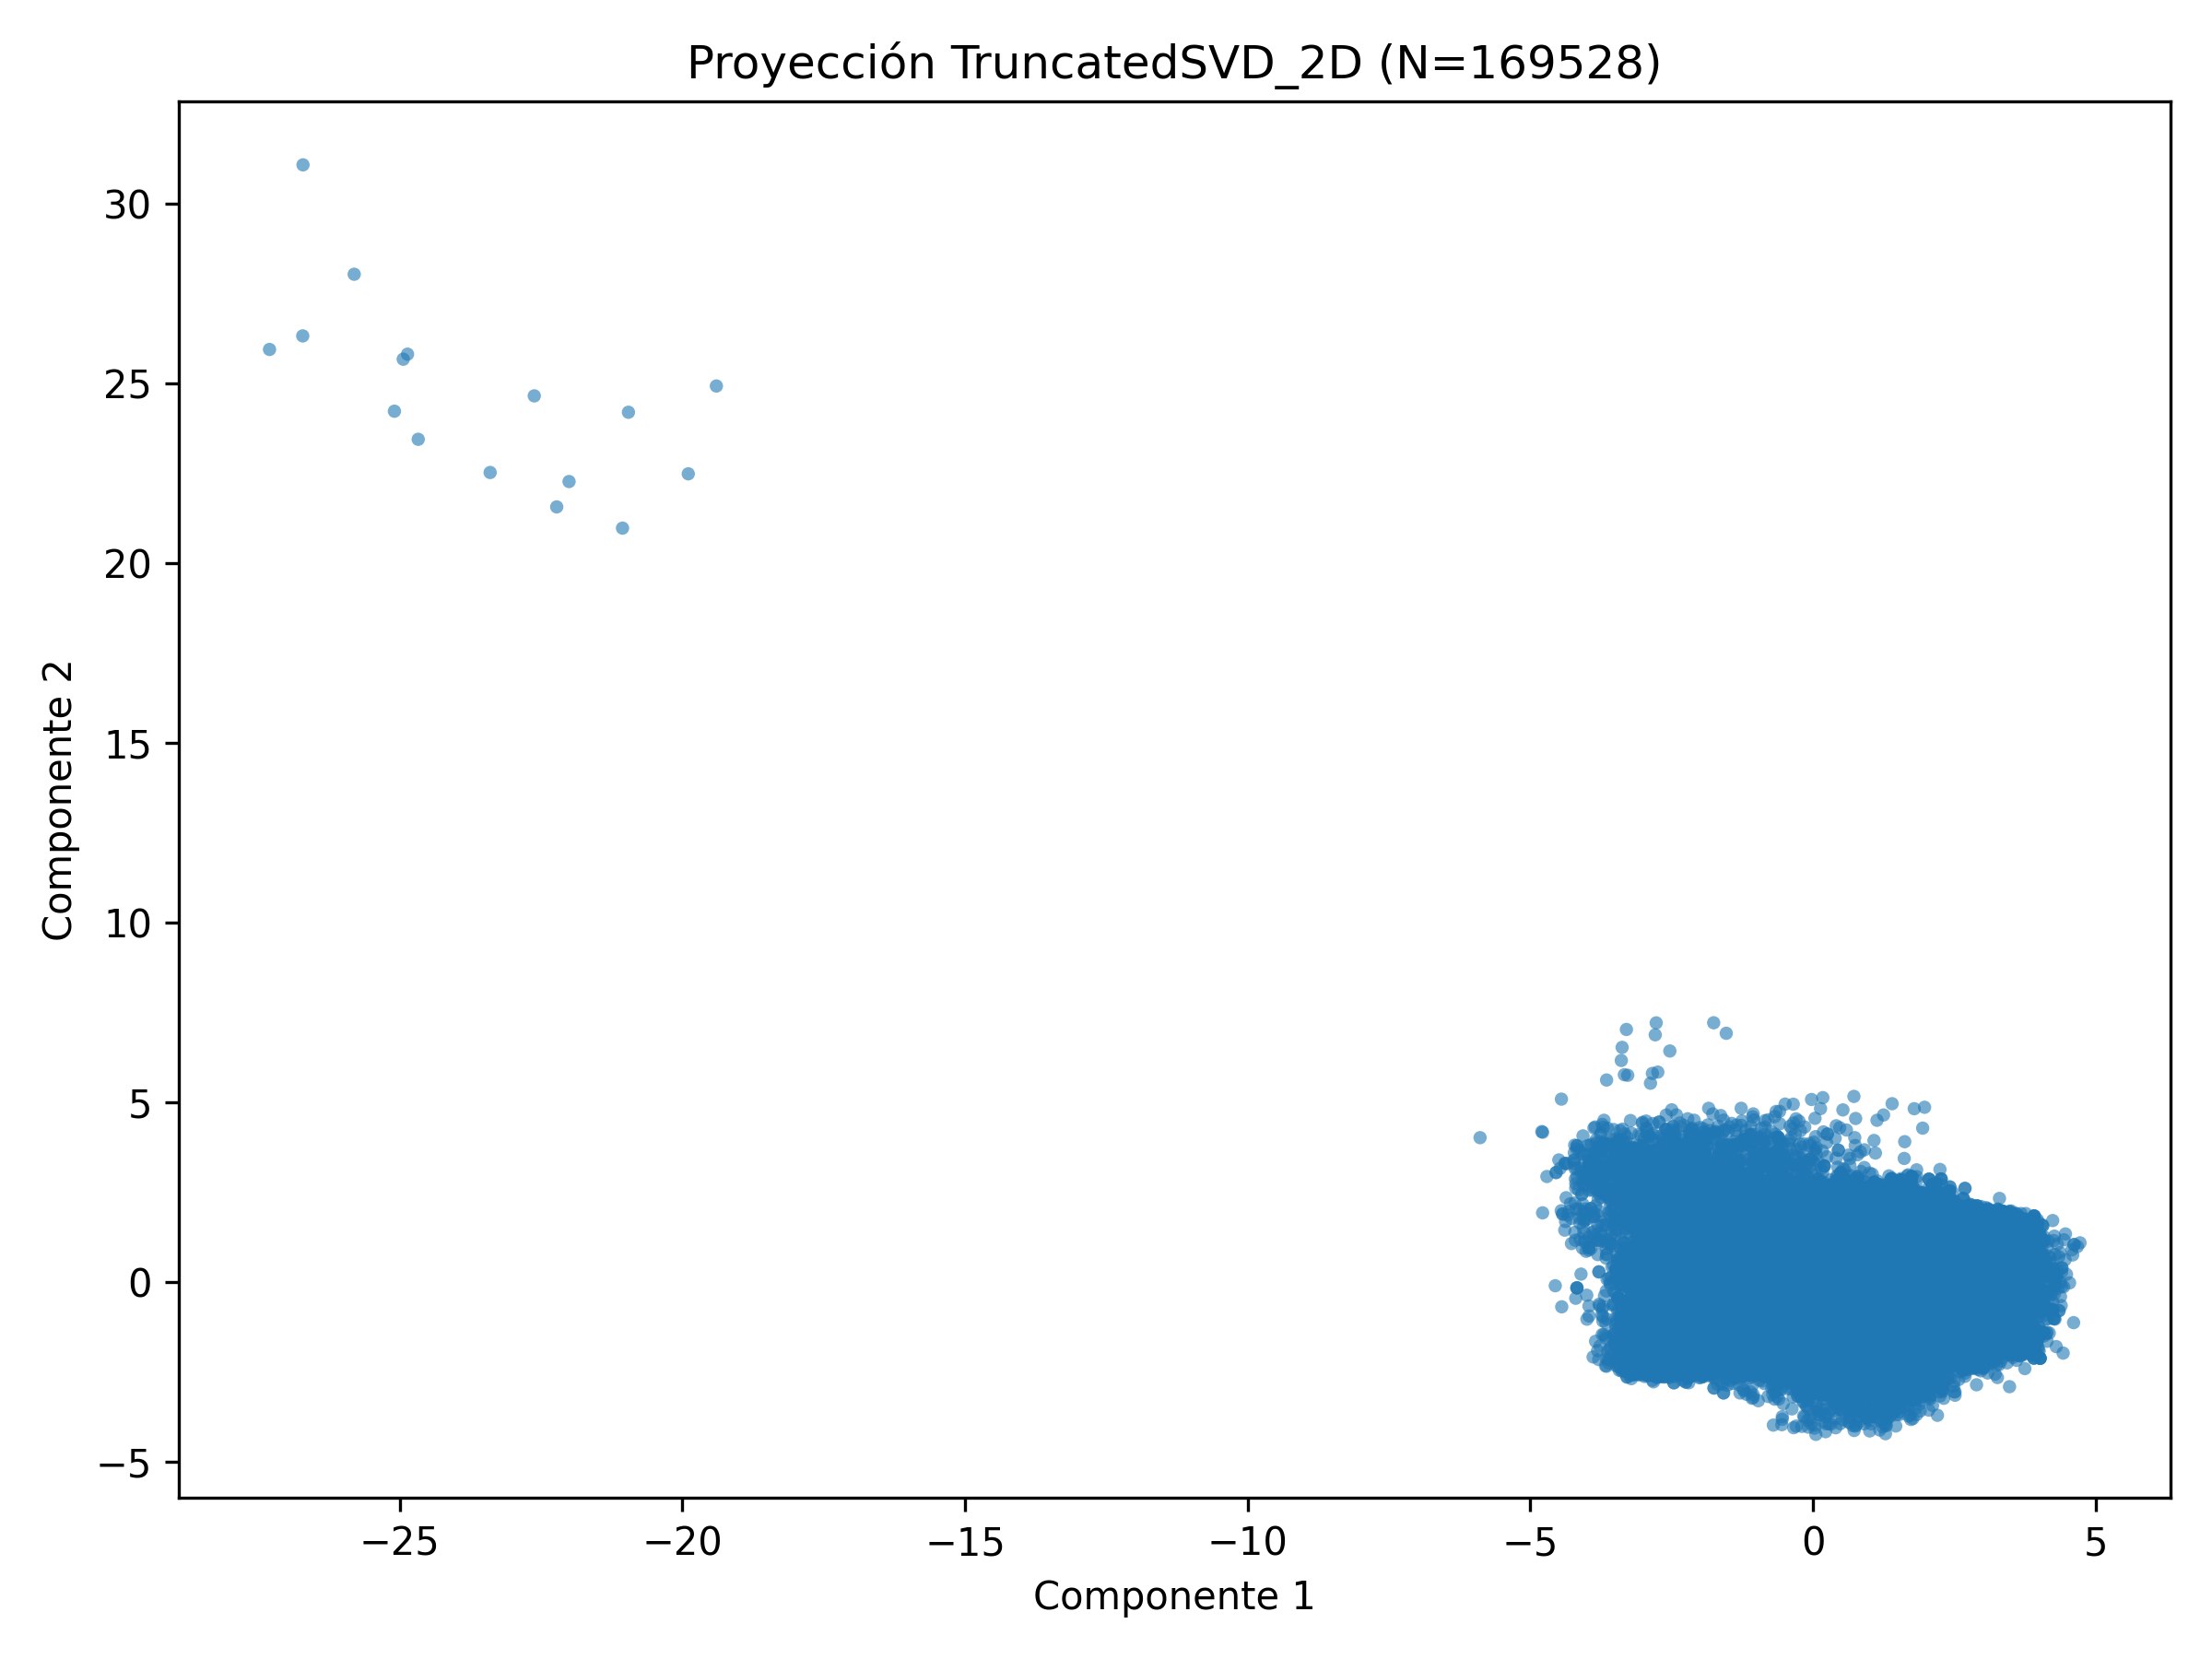
\includegraphics[width=\textwidth, height=0.75\textheight, keepaspectratio]{plot_TruncatedSVD_2D.png}
      \caption{\small Proyección Truncated SVD 2D}
    \end{figure}
    
    \column{0.50\textwidth}
    \begin{figure}
      \centering
      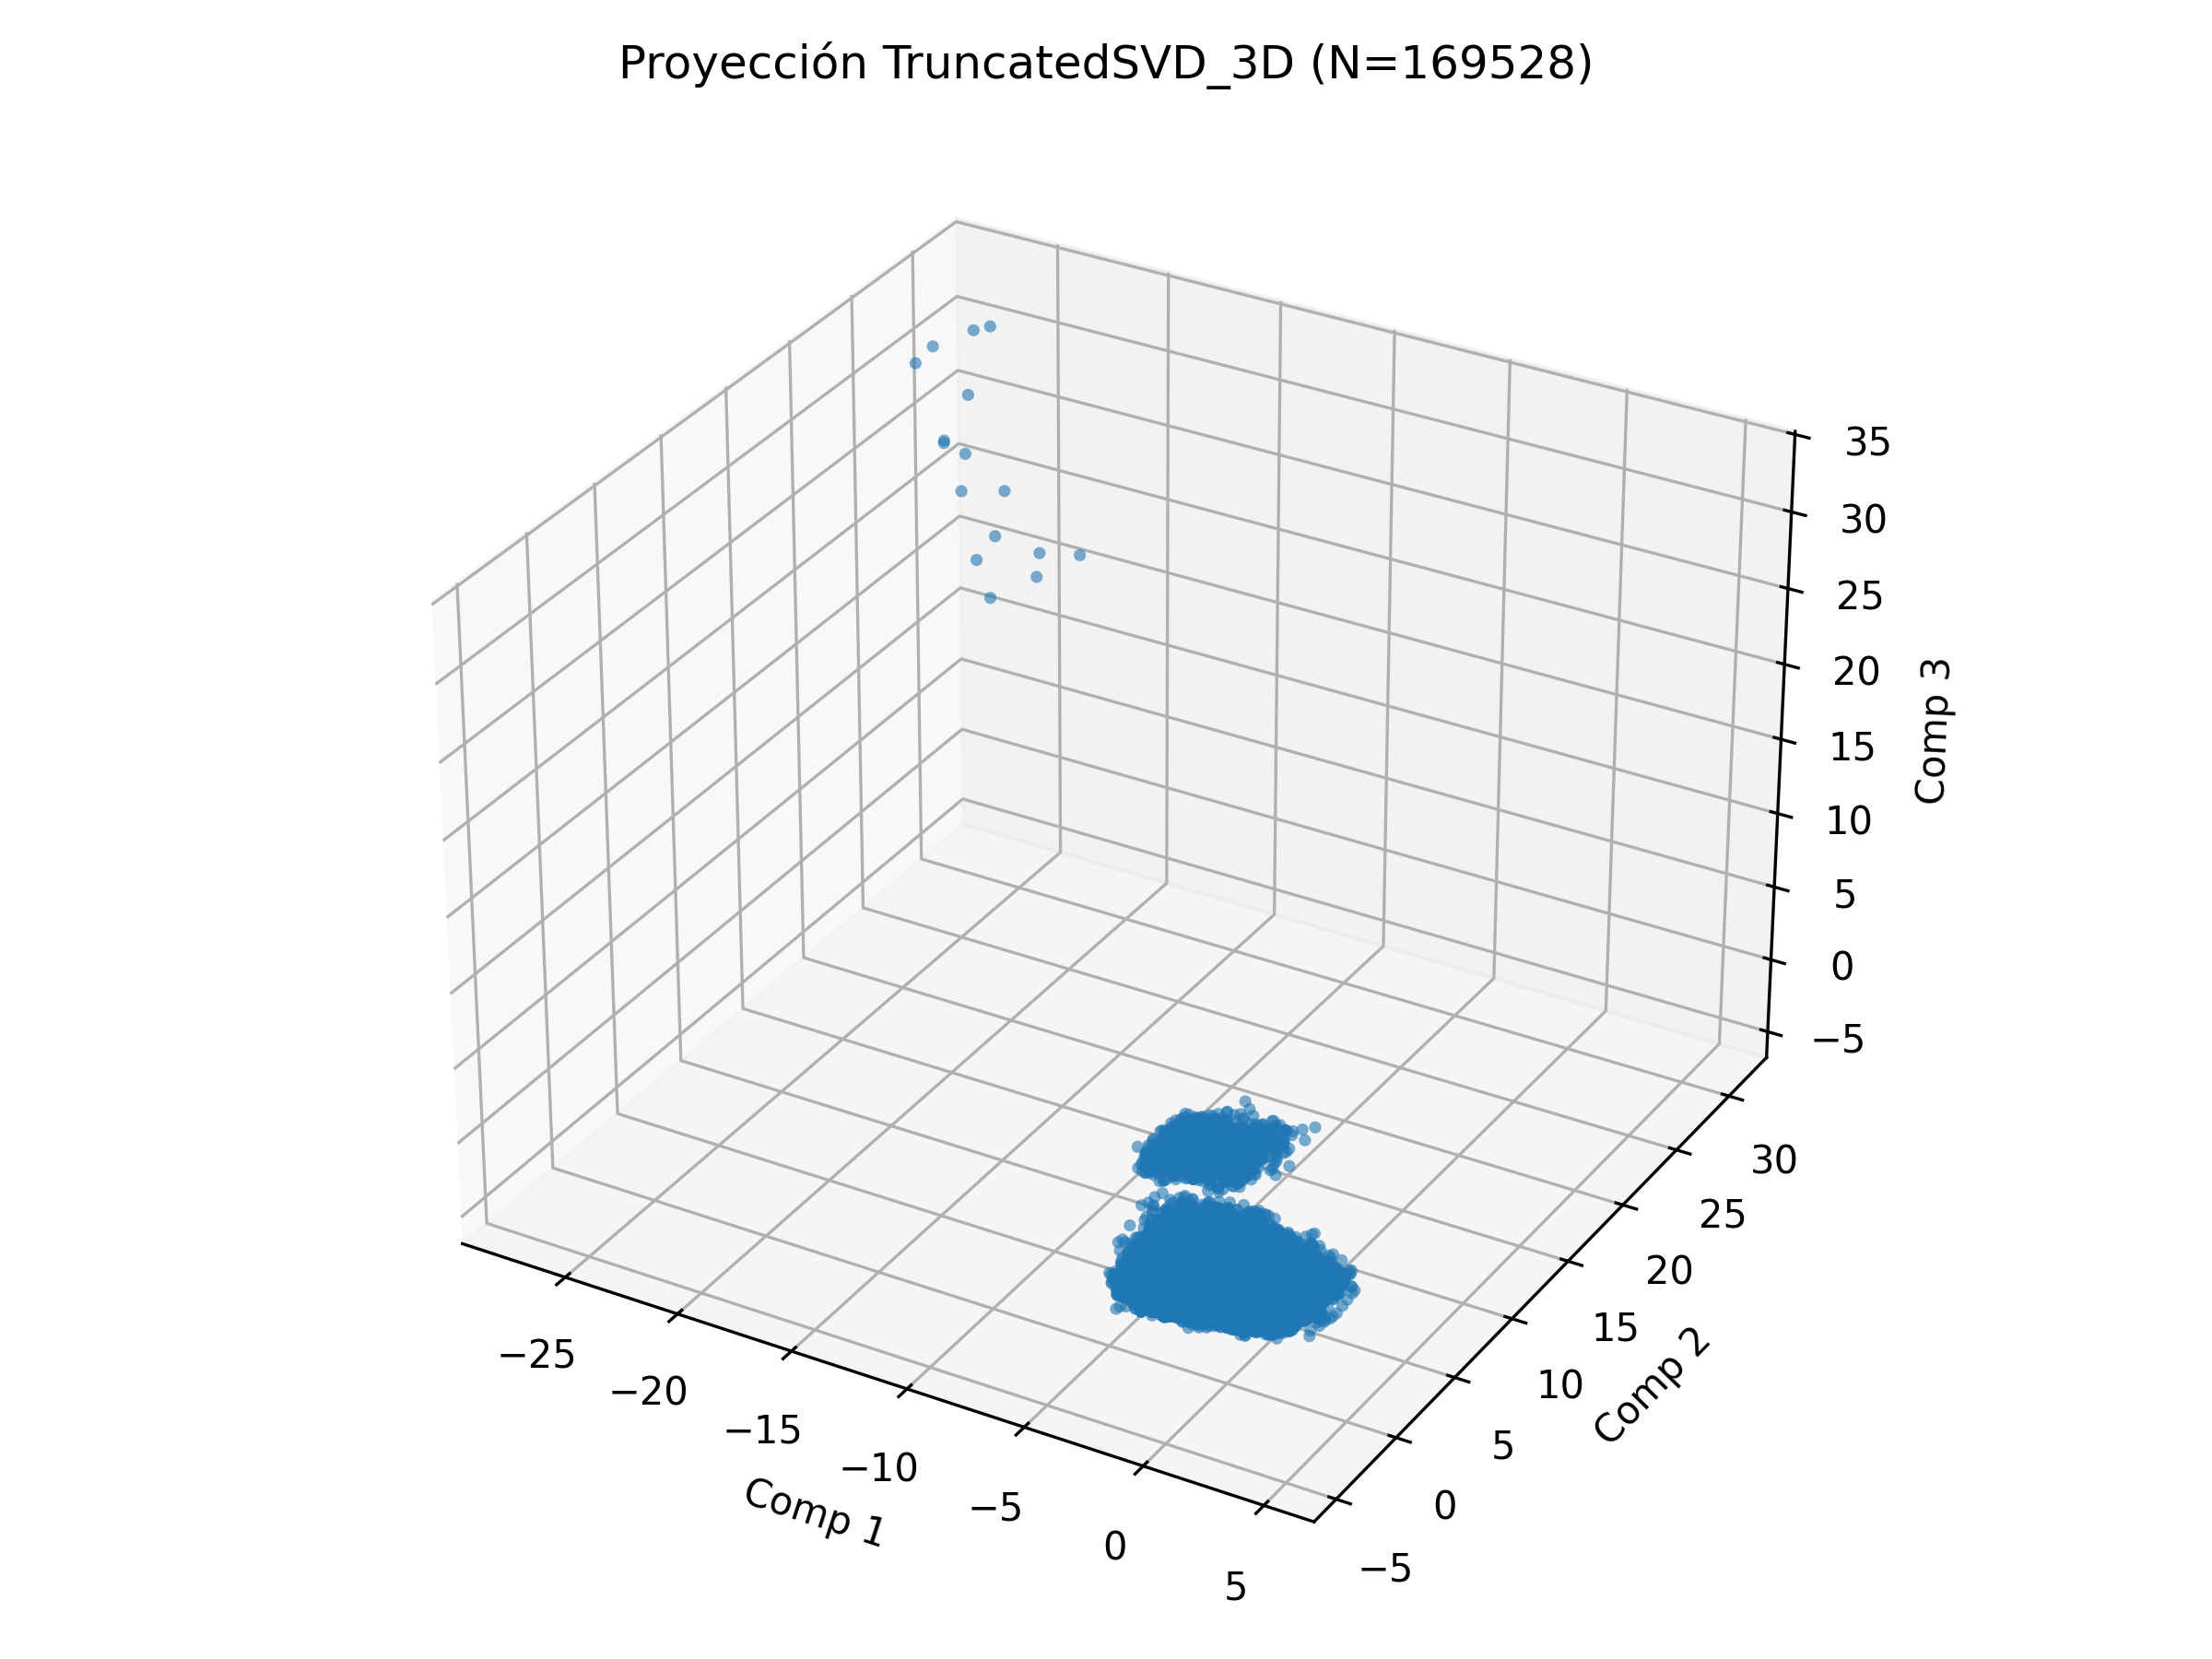
\includegraphics[width=\textwidth, height=0.75\textheight, keepaspectratio]{plot_TruncatedSVD_3D.png}
      \caption{\small Proyección Truncated SVD 3D}
    \end{figure}
  \end{columns}
\end{frame}

\begin{frame}[c]
  \centering
  \vspace{1cm}

  \begin{block}{}
    \centering
    \Large \texttt{Process exited with code 0 (EOF)}
  \end{block}

  \vspace{0.8cm}

  {\Huge \textbf{¡Muchas gracias por su atención!}}

  \vspace{0.8cm}

  \begin{columns}
    \column{0.8\textwidth}
    \centering
    \small
    \texttt{\# Preguntas \& Comentarios}\\
    \texttt{std::cout << "Q\&A Session Opened" << std::endl;}
  \end{columns}
\end{frame}


\end{document}
